\subsection{IFIT1, IFIT3, and IFIT5 Localisation with Regards to RSV Pseudo-IBs} \label{subsec:IFIT1, IFIT3, and IFIT5 Localisation with Regards to RSV Pseudo-IBs}


To investigate the intreaction of IFITs with RSV pseudo inclusion bodies ...

The cells, regardless of the cell line used were cultured and passaged using the standard conditions and procedures, as decribed in Sections \ref{sec:Cell Culture} and \ref{subsec:Passaging and Seeding Cells}. Human or bovine RSV N or P codon optimised ORFs, which were situated in pcDNA3.1 plasmid backbones, were transfected into the cells using TransIT-X2 in 1:2 ratio, as decribed in Section \ref{subsec:Transfecting Cells}. We have tried transfection with lipofectamine 3000 as well, although it was more toxic to cells and provided smilar transfection efficiencies (data not shown). After trying and optimising the transfection conditions in terms of total DNA used, seeding density and different ratios of RSV N and P containing plasmids (data not shown), we have ended up consistently transfecting 500 $\mu$g of each plasmid per 50k cells seeeded in 24 well plate per well.

The initial experiments were conducted in human embryonic kidney (HEK) 293T cells, which were very persmisive to plasmid transfection and oftern displaying transfection efficiencies of >90\%. They are not really suitable for confocal microscopy and subsequent image analysis as they have small nucleus to cytoplasm ratio. They are also dfficult to work with as they easily detach from the plastic culture plates during treatment or washes. Regardless, the initial IFIT1 and IFIT2 (Section \ref{subsec:Dissecting the Differential IFIT2 Antibody Staining}) staining experiments were conducted using these cells. Due to this we have transitioned into other cell lines. We have tested HeLa and Vero cell lines based on their transfection permisivity, cell morphology, and ease of culture. HeLa was more suitable based on its origin (human uterine epithelial cancer cell line), while the Vero cell line is derived from kidney epithelial tissue of adult African green monkey (\textit{Cercopithecus aethiops}) \cite{Simizu1967CharacterizationVero}. Initial optimasition showed minimal transfection in HeLa cell line in each of the condition tested (data not shown), while the Vero cells were showing constant transfection, albeit with lower transfection efficiencies than what we observed in HEK293T cell line (circa 30\%/90\%, data not shown). Regardless, this was sufficient for confocal microscopy experiments.

Vero cells are ruitinely used to propagate and study a range of viruses, espoecially bRSV. Althogh it would be optimal to be detecting endogenous human IFITs interacting with RSV pseudo-IBs, IFITs of primates are phylogenetically more closely related to human IFITs that bovine IFITs \cite{Zhou2013InterferonDefense.}. Additionaly we have observed in the previous chapter that the interactions of human and bovine IFITs are fairly consistend. Thus assesing the monkey IFIT colocalisation with human or bovine pIBs could yield useful insights into the matter.

\begin{figure}
    \begin{subfigure}{0.495\textwidth}
        \caption{}
        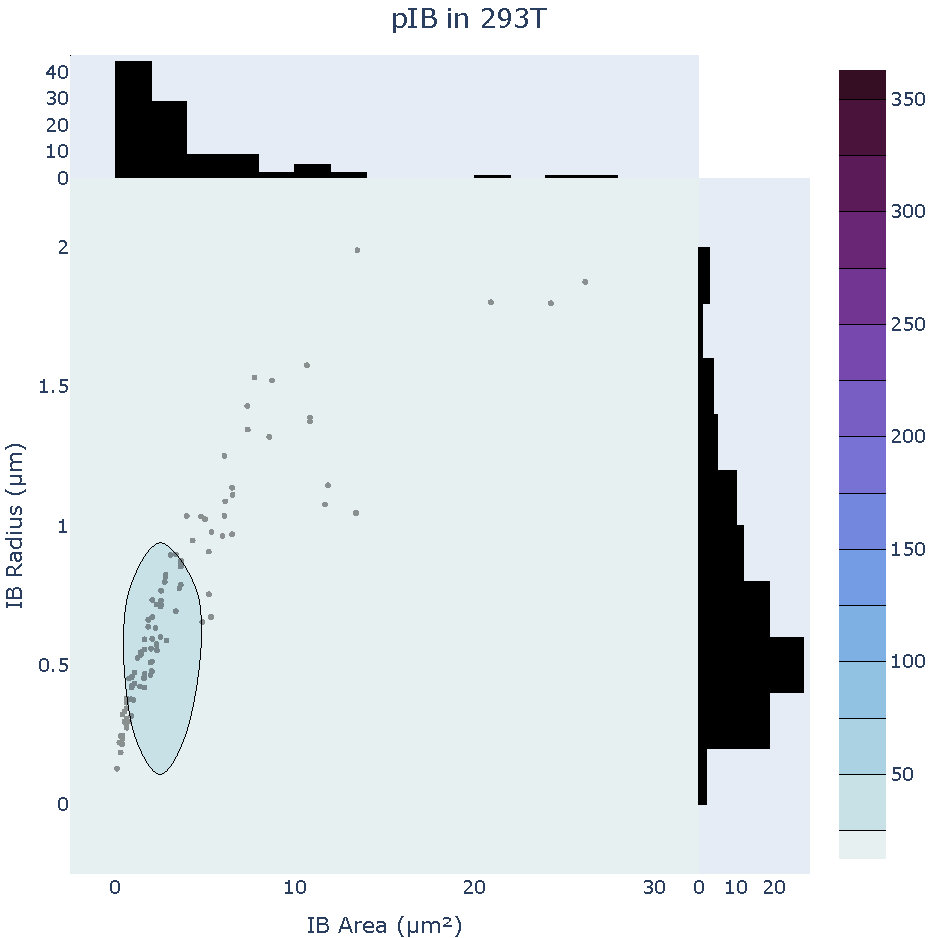
\includegraphics[width=\textwidth]{09. Chapter 4/Figs/01. pIB/01. pIB characterisation/01. heatmap_pib-293t.pdf} 
    \end{subfigure}
    \hfill
    \begin{subfigure}{0.495\textwidth}
        \caption{}
        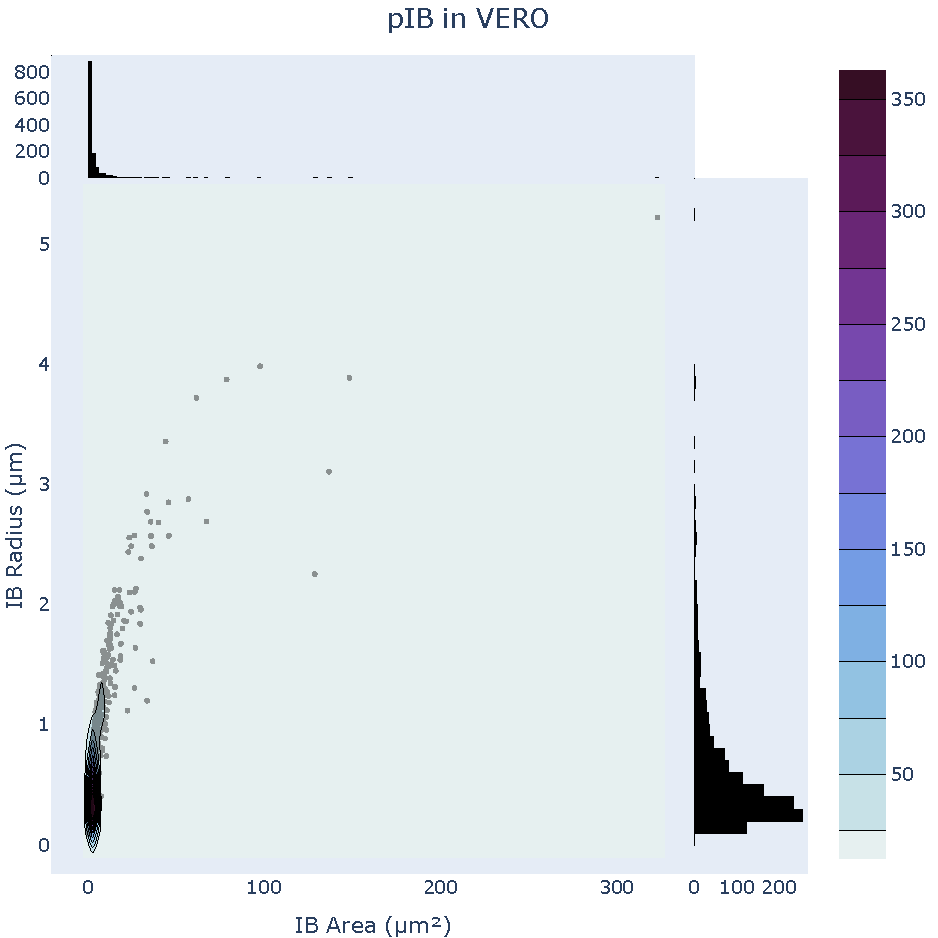
\includegraphics[width=\textwidth]{09. Chapter 4/Figs/01. pIB/01. pIB characterisation/02. heatmap_pib-vero.pdf}
    \end{subfigure}
    \caption[Size Characterisation of Pseudo Inclusion Bodies Across Different Cell Lines.]{\textbf{Size Characterisation of Pseudo Inclusion Bodies Across Different Cell Lines.} This figure presents the relationship between the measured area (\(\mu \mbox{m}^2\)) and diameter (\(\mu \mbox{m}\)) of individual pseudo inclusion bodies (pIBs) as observed within the scope of this study. Additionally, the figure includes distinct population distributions depicted alongside the plots, representing (a) 103 observations from the 293T cell line and (b) 1321 observations from the Vero cell line. Contour plots are incorporated to elucidate the underlying density of individual IBs within the plots.}
    \label{fig:Size Characterisation of Pseudo Inclusion Bodies Across Different Cell Lines}
\end{figure}

We systematically observed and annotated a total of 1424 pseudo inclusion bodies across HEK293T (103 observations) and Vero (1321 observations) cell lines. The relationship between their measured area and radia can be observed in Figure \ref{fig:Size Characterisation of Pseudo Inclusion Bodies Across Different Cell Lines}. pIBs observed in both cell lines broadly follow logaritmic curves, as expected based on the relationship of the observed values, although we can observe a sizable number of detected entities that show larger measured area compared to predicted radius. This indicates elongated ellipsioid shape. The pIBs detected in 293T cell line mainly exhibited the radia of 0.5 \(\mu \mbox{m}\), with the majority of the detected pIBs having their radia between 0.25 \(\mu \mbox{m}\) and 1 \(\mu \mbox{m}\). With regards to their associated measured area, most of the pIBs were between 0.5 \(\mu \mbox{m}^2\) and 4 \(\mu \mbox{m}^2\). In the Vero cell line we can observe a higher spread of data as we have observed pIB measuring >5 \(\mu \mbox{m}\) in radius and >300 \(\mu \mbox{m}^2\), however, majoprity of the detrected entities confronted to radia between 0.1 \(\mu \mbox{m}\) and 0.7 \(\mu \mbox{m}\), with the measured 2D area betweeen 0.1 \(\mu \mbox{m}^2\) and 4 \(\mu \mbox{m}^2\).

\begin{figure}
    \centering
    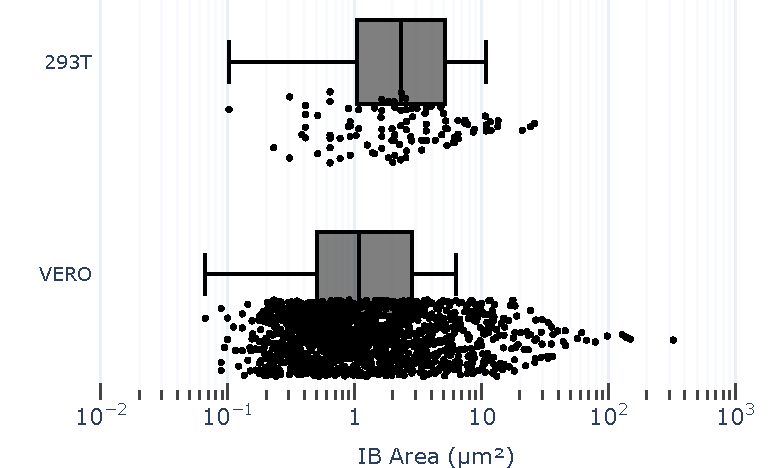
\includegraphics[width=0.75\linewidth]{09. Chapter 4/Figs/01. pIB/01. pIB characterisation/03. box-pib.pdf}
    \caption[The Distributions of pIB Areas Observed Per Cell Line.]{\textbf{The Distributions of pIB Areas Observed Per Cell Line.} The distribution of RSV pseudo inclusion body areas (\(\mu \mbox{m}^2\)), detected in this study are shown. A total of 103 observations were made in the 293T cell line, and 1321 observations in the Vero cell line.}
    \label{fig:The Distributions of pIB Areas Observed Per Cell Line}
\end{figure}

A more detailed view focusong solely on the distribution of measured areas per cell line can be observed in Figure \ref{fig:The Distributions of pIB Areas Observed Per Cell Line}. We can see that pIBs detected in Vero cell line encompas larger range in terms of the minimal and maximal measured area copared to the 293T cell line, however, the median value in the latter was higher. In more detal, in 293T cell line we have measured pIB areas ranging from sub 0.2 \(\mu \mbox{m}^2\) to supra 20 \(\mu \mbox{m}^2\), with the median value of 2.2 \(\mu \mbox{m}^2\), while in Vero cell line we have observed pIBs ranging from sub 0.07 \(\mu \mbox{m}^2\) to supra 300 \(\mu \mbox{m}^2\), with the median value of 1 \(\mu \mbox{m}^2\). Both median values are considerably smaller to what was observed in cell lines during infection (Section \ref{subsec:IFIT Subcellular Localisation During Interferon Induction and RSV Infection}, Figure \ref{fig:The Distributions of IB Areas Observed Per Cell Line}), which is in line to what was reported in literature where pIBs observed 24 hours post-transfection were considerably smaller than conventional IBs observed in infected cells after equivalent passage of time cite{Jobe2021BovineResponses}.

\begin{figure}
    \begin{subfigure}{0.495\textwidth}
        \caption{}
        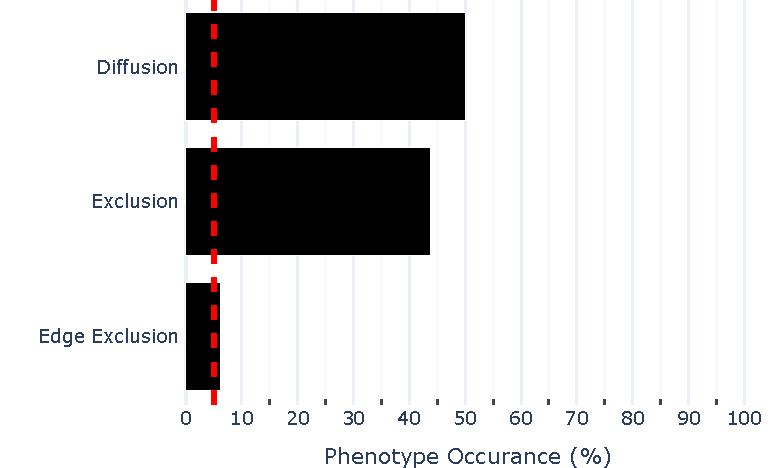
\includegraphics[width=1\linewidth]{09. Chapter 4/Figs/01. pIB/02. IFIT1/01. bar_i1_293t.pdf} 
    \end{subfigure}
    \begin{subfigure}{0.495\textwidth}
        \caption{}
        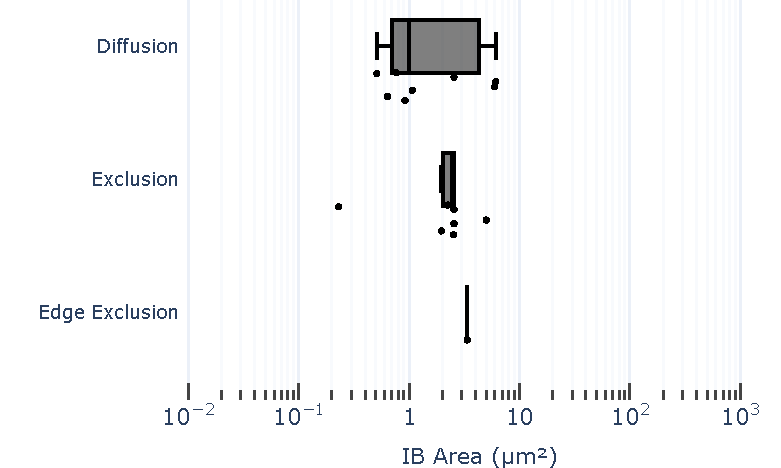
\includegraphics[width=1\linewidth]{09. Chapter 4/Figs/01. pIB/02. IFIT1/02. box_i1_293t.pdf}
    \end{subfigure}
    \caption[Phenotypic Interactions of Human IFIT1 with Human pIBs in the 293T Cell Line.]{\textbf{Phenotypic Interactions of Human IFIT1 with Human pIBs in the 293T Cell Line.} 293T cells were transfected with hRSV N and P containing plasmids using TransIT-X2 and were fixed after 24 hours. Cells were labeled with anti-RSV N and anti-IFIT1 antibodies and imaged on confocal microscope. Panel (a) shows percentual proportions of observed phenotypes between hRSV pseudo inclusion bodies and human IFIT1 (16 observations), with the red dotted line denoting the 5\% threshold, marking phenotypes considered relevant above this limit. Panel (b) shows the IB area in \(\mu \mbox{m}^2\) per observed relevant phenotype.}
    \label{fig:Phenotypic Interactions of Human IFIT1 with Human pIBs in the 293T Cell Line}
\end{figure}

\begin{figure}
    \centering
    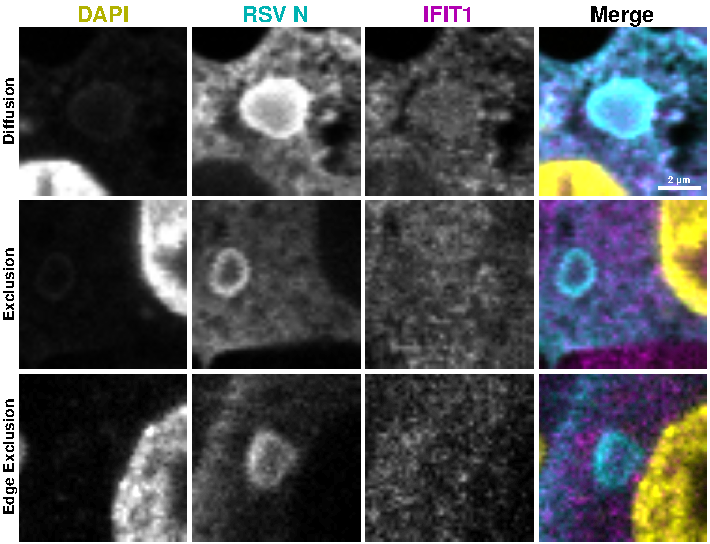
\includegraphics[width=1\linewidth]{09. Chapter 4/Figs/01. pIB/02. IFIT1/03. i1-293t-hnhp.pdf}
    \caption[Representative Images of Phenotypic Interactions of Human IFIT1 with Human pIBs in the 293T Cell Line.]{\textbf{Representative Images of Phenotypic Interactions of Human IFIT1 with Human pIBs in the 293T Cell Line.} 293T cells were transfected with hRSV N and P containing plasmids using TransIT-X2 and were fixed after 24 hours. Cellular nuclei were stained with DAPI (yellow), and cells were double-labeled with anti-RSV N (cyan) and anti-IFIT1 (magenta) antibodies. This figure showcases representative examples of relevant phenotypes in the interaction between human IFIT1 and hRSV pseudo inclusion bodies. These phenotypes are presented in descending order based on their percentage proportions. The scale bar indicates 2 \(\mu \mbox{m}\).}
    \label{fig:Representative Images of Phenotypic Interactions of Human IFIT1 with Human pIBs in the 293T Cell Line}
\end{figure}


We obtained 16 observations of endogenous human IFIT1 and its interaction with hRSV pIBs in 293T cell line. The observed phenotype frequencies, along with the measured pIB sizes can be vewed n Figure \ref{fig:Phenotypic Interactions of Human IFIT1 with Human pIBs in the 293T Cell Line}, with the representative iimagese of these phenotypes shown in Figure \ref{fig:Representative Images of Phenotypic Interactions of Human IFIT1 with Human pIBs in the 293T Cell Line}. A half of the observations displayed diffusion phenotype. This was predominantly observed in smaller pIBs with a typical size of 1 \(\mu \mbox{m}^2\) and ranging from 0.5 \(\mu \mbox{m}^2\) to 6 \(\mu \mbox{m}^2\) in size. The second most prevalent phenotype was exclusion, which occured in 44\% of cases. The pIBs associatred with this phenotype closely clustered at around 2.5 \(\mu \mbox{m}^2\), whith two exceptions i.e. one very small pIB (0.22 \(\mu \mbox{m}^2\)) and one ralitaively large pIB (5 \(\mu \mbox{m}^2\)). Lastly, we have observed one pIB with a measured area of 3.3 \(\mu \mbox{m}^2\) which exhibited size exclusion phenotype. Overall these data suggest human IFIT1 not associating with human RSV pIB structures, although this is based on a very limited set of observations.

\begin{figure}
    \begin{subfigure}{0.495\textwidth}
        \caption{}
        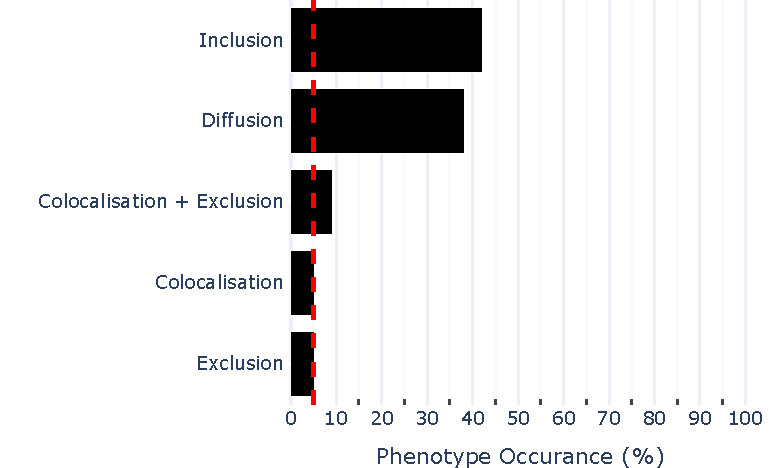
\includegraphics[width=1\linewidth]{09. Chapter 4/Figs/01. pIB/02. IFIT1/04. bar_i1_vero_hnhp.pdf} 
    \end{subfigure}
    \begin{subfigure}{0.495\textwidth}
        \caption{}
        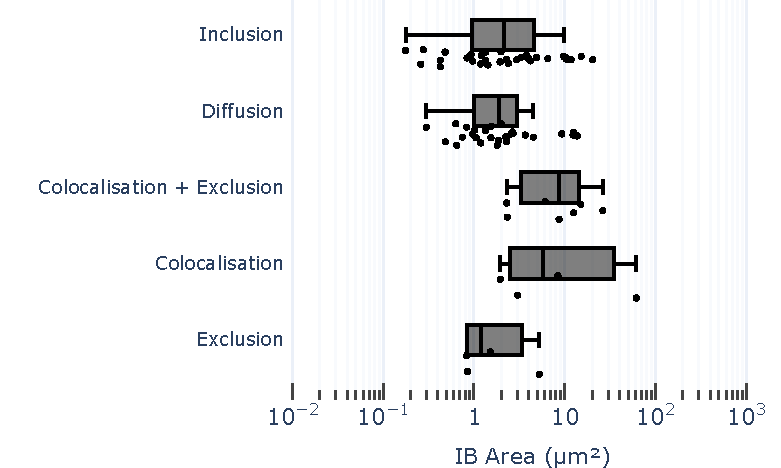
\includegraphics[width=1\linewidth]{09. Chapter 4/Figs/01. pIB/02. IFIT1/05. box_i1_vero_hnhp.pdf}
    \end{subfigure}
    \caption[Interaction Phenotypes of Monkey IFIT1 with Human pIBs in the Vero Cell Line.]{\textbf{Interaction Phenotypes of Monkey IFIT1 with Human pIBs in the Vero Cell Line.} Vero cells were transfected with hRSV N and P containing plasmids using TransIT-X2 and were fixed after 24 hours. Cells were labeled with anti-RSV N and anti-IFIT1 antibodies and imaged on confocal microscope. Panel (a) shows percentual proportions of observed phenotypes between hRSV pseudo inclusion bodies and monkey IFIT1 (76 observations), with the red dotted line denoting the 5\% threshold, marking phenotypes considered relevant above this limit. Panel (b) shows the IB area in \(\mu \mbox{m}^2\) per observed relevant phenotype.}
    \label{fig:Interaction Phenotypes of Monkey IFIT1 with Human pIBs in the VERO Cell Line}
\end{figure}

\begin{figure}
    \centering
    \includegraphics[width=1\linewidth]{09. Chapter 4/Figs/01. pIB/02. IFIT1/06. i1-vero-hnhp.pdf}
    \caption[Representative Images of Interaction Phenotypes of Monkey IFIT1 with Human pIBs in the Vero Cell Line.]{\textbf{Representative Images of Interaction Phenotypes of Monkey IFIT1 with Human pIBs in the Vero Cell Line.} Vero cells were transfected with hRSV N and P containing plasmids using TransIT-X2 and were fixed after 24 hours. Cellular nuclei were stained with DAPI (yellow), and cells were double-labeled with anti-RSV N (cyan) and anti-IFIT1 (magenta) antibodies. This figure showcases representative examples of relevant phenotypes in the interaction between monkey IFIT1 and hRSV pseudo inclusion bodies. These phenotypes are presented in descending order based on their percentage proportions. The scale bar indicates 2 \(\mu \mbox{m}\).}
    \label{fig:Representative Images of Interaction Phenotypes of Monkey IFIT1 with Human pIBs in the VERO Cell Line}
\end{figure}

Next we have evaluated endogenous monkey IFIT1 interactions with pIBs created by transfection of hRSV N and P proteins in Vero cell line. The frequencies of occurances of the interaction phenotypes based on 76 observations, along with the measured pIB areas per phenotype are shown in Figure \ref{fig:Interaction Phenotypes of Monkey IFIT1 with Human pIBs in the VERO Cell Line}. The representative images of these phenotypes are shown in Figure \ref{fig:Representative Images of Interaction Phenotypes of Monkey IFIT1 with Human pIBs in the VERO Cell Line}. 43\% of the observations show monkey IFIT1 forming intra pIB inclusion. This was followed by a diffusion phenotype, which occured in 38\% of observations. Further, 8\% of the observations showed monkey IFIT1 to be colocalisiong with the edge of the pIB structure while beiing excluded from the main pIB structure. Lastly, colocalisation and exclusion phenotypes both individually occured in 5\% of cases each. With regards to the size profile of hRSV pIBs associated with these phenotypes, inclusion was observed in a wide range of pIB sizes, ranging from sub 0.2 \(\mu \mbox{m}^2\) to supra 20 \(\mu \mbox{m}^2\) with a median size of 2 \(\mu \mbox{m}^2\). The diffusion phenotype was observed in pIBs with a smilar range of measured areas, with an identical median value of 2 \(\mu \mbox{m}^2\). These two phenotypes differ in the distribution of their values. While the pIB sizes of inclusion phenotype-associated pIBs were evenly distributed between its minimal and maximal values, diffusion-associated pIBs clustered at around 2 \(\mu \mbox{m}^2\). The colocalisation associated with pIB exclusion phenotype occured in larger pIBs with the typical area of 9 \(\mu \mbox{m}^2\) and was not observed in pIBs which were smaller than 2 \(\mu \mbox{m}^2\). The colocalisation-phenotype associated hRSV pIBs as well were of larger size, with the median value of 6 \(\mu \mbox{m}^2\), and minimal value of 2 \(\mu \mbox{m}^2\). Lastly the exclusion phenotype was was observed to be associated with 4 pIBs which had median 2D area of 1.1 \(\mu \mbox{m}^2\). Overall, although in this simplified model, the size of the pIB should not directly mean a difference in the underlying pIB complexity. Regardelss we observe size-dependent phenotype association. In smaller, sub 1 \(\mu \mbox{m}^2\) pIBs we only observed inclusiohn and diffusiion phenotyeps, which were equally prevelant in these. Larger pIBs had inclusion, diffusion and colocalisation associated with exclusion associated with them.

\begin{figure}
    \begin{subfigure}{0.495\textwidth}
        \caption{}
        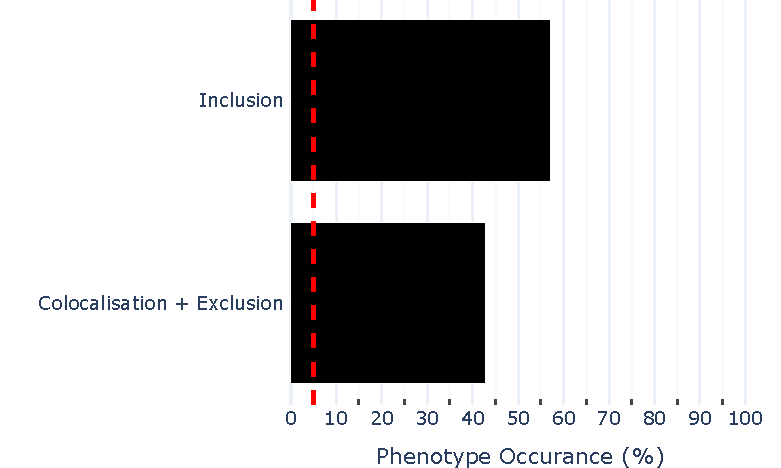
\includegraphics[width=1\linewidth]{09. Chapter 4/Figs/01. pIB/02. IFIT1/07. bar_i1_vero_bnbp.pdf}  
    \end{subfigure}
    \begin{subfigure}{0.495\textwidth}
        \caption{}
        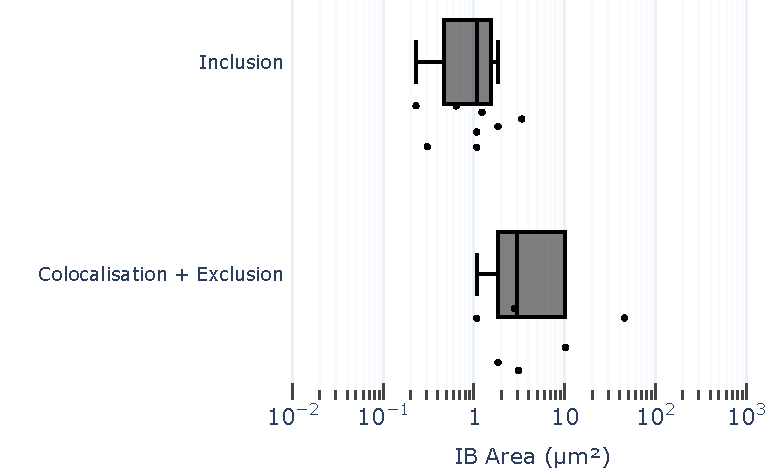
\includegraphics[width=1\linewidth]{09. Chapter 4/Figs/01. pIB/02. IFIT1/08. box_i1_vero_bnbp.pdf}
    \end{subfigure}
    \caption[Interaction Phenotypes of Monkey IFIT1 with Bovine pIBs in the Vero Cell Line.]{\textbf{Interaction Phenotypes of Monkey IFIT1 with Bovine pIBs in the Vero Cell Line.} Vero cells were transfected with bRSV N and P containing plasmids using TransIT-X2 and were fixed after 24 hours. Cells were labeled with anti-RSV N and anti-IFIT1 antibodies and imaged on confocal microscope. Panel (a) shows percentual proportions of observed phenotypes between bRSV pseudo inclusion bodies and monkey IFIT1 (14 observations), with the red dotted line denoting the 5\% threshold, marking phenotypes considered relevant above this limit. Panel (b) shows the IB area in \(\mu \mbox{m}^2\) per observed relevant phenotype.}
    \label{fig:Interaction Phenotypes of Monkey IFIT1 with Bovine pIBs in the VERO Cell Line}
\end{figure}

\begin{figure}
    \centering
    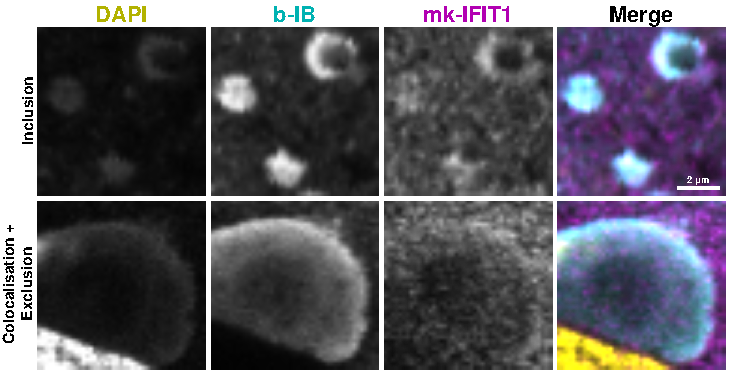
\includegraphics[width=1\linewidth]{09. Chapter 4/Figs/01. pIB/02. IFIT1/09. i1-vero-bnbp.pdf}
    \caption[Representative Images of Interaction Phenotypes of Monkey IFIT1 with Bovine pIBs in the Vero Cell Line.]{\textbf{Representative Images of Interaction Phenotypes of Monkey IFIT1 with Bovine pIBs in the Vero Cell Line.} Vero cells were transfected with bRSV N and P containing plasmids using TransIT-X2 and were fixed after 24 hours. Cellular nuclei were stained with DAPI (yellow), and cells were double-labeled with anti-RSV N (cyan) and anti-IFIT1 (magenta) antibodies. This figure showcases representative examples of relevant phenotypes in the interaction between monkey IFIT1 and bRSV pseudo inclusion bodies. These phenotypes are presented in descending order based on their percentage proportions. The scale bar indicates 2 \(\mu \mbox{m}\).}
    \label{fig:Representative Images of Interaction Phenotypes of Monkey IFIT1 with Bovine pIBs in the VERO Cell Line}
\end{figure}

Lastly we have observed monkey IFIT1 interaction,detected by human IFIT1 antibody, with bovine RSV pIBs, using the transfection of bRSV N and P containing plasmids. These plasmids consistently yielded lower transfection efficiencies and thus posed difficulties in obtaining a large amount of observations. Due to this we have failed to generate enough samples to investigate endogenous monkey IFTIs other than IFIT1 and IFIT2using the A antibody (with the respective results shown and discussed in Section \ref{subsec:Dissecting the Differential IFIT2 Antibody Staining}). Regardless, the frequencies of occurances of the interaction phenotypes based on 14 observations, along with the measured pIB areas per phenotype are shown in Figure \ref{fig:Interaction Phenotypes of Monkey IFIT1 with Bovine pIBs in the VERO Cell Line}. The representative images of these phenotypes are shown in Figure \ref{fig:Representative Images of Interaction Phenotypes of Monkey IFIT1 with Bovine pIBs in the VERO Cell Line}. We can observe results reminiscent of what was observed with IFIT2, detected by IFIT2(A) antibody during RSV infectrion. That is we observe only two phenotypes: inclusion within the pIB structures, which occurs at 56\% frequency and colocalisation associated with pIB exclusion, which occurs at 44\% frequency. The former occurs predominantly in smaller pIBs, with the median size of 1 \(\mu \mbox{m}^2\) and not bigger than 4 \(\mu \mbox{m}^2\). On the other hand, the colocalisation phenotype associated with exclusion occurs in pIBs with a typical size of 3 \(\mu \mbox{m}^2\). There is an overlap between the pIB sizes of the two phenotypes, although sub 1 \(\mu \mbox{m}^2\) pIBs are always associated with inclusion while supra 10 \(\mu \mbox{m}^2\) are always associated with colocalisation cojoined with exclusion.

Taking all of the IFIT1-pIB interaction results together it seems like there is a differential propensity for pIB interaction between endogenous human and monkey IFIT1. Saying that, data obtained from HEK293T cell line is limited in quantity and displays a size bias towards pIBs that are less than 6 \(\mu \mbox{m}^2\) in size. This does not correspond to the true diversity of pIB sizes observed in this study as the aggregate 293T suggest there is a sizable population of supra 6 \(\mu \mbox{m}^2\) pIBs that was detected in this study (Figure \ref{fig:The Distributions of pIB Areas Observed Per Cell Line}). In the Vero cell line transfected with hRSV N and P ORF-containing plasmids, we have observed phenotypes that imply direct interaction (colocalisation and colocalisation asssociated with exclusion) specificaly in larger pIBs. This implies that the limited sample size and diversity in 293T observed hRSV pIBs is not sufficient to provide true picture of IFIT1/pIB interaction. On the other hand, it can be also implicative of hIFIT1 not being recruited to the pIBs. Within the Vero cell line we also ofbserved differential results which dependent on the species of the virus. While we have only observed direct interaction phenotypes of inclusion formation and pIB edge colocalsiation with intra-pIB exclusion with the bRSV pIBs, we observed a more diverse interaction range in Vero cells with hRSV pIBs present in them. These phenotypes, however, all, with the exeption of exclusion phenotype (which occured only in 5\% of observations), implied IFIT1 having access to the pIB structure. It is intrueegin to see the differences between humand and bovine RSV pIB and their interaction with monkey IFIT1. This could suggest that the bovine pIB possibly lack mechanism that would prevent them from being targeted by the moneky IFIT1. Saying that, the bovine RSV pIB dataset lacks inthe depth with regards to the amount of observations, and thus the differences could also be atributed to low frequency of diffusion or exclusion phenotypes. In that case the results from Vero cell lines with either human or bovine RSV pIBs present would be almost identical.

\begin{figure}
    \begin{subfigure}{0.495\textwidth}
        \caption{}
        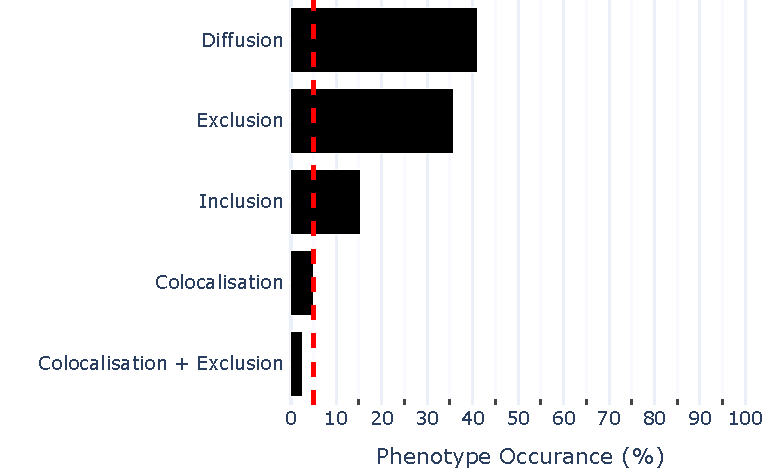
\includegraphics[width=1\linewidth]{09. Chapter 4/Figs/01. pIB/04. IFIT3/01. bar_i3_vero.pdf} 
    \end{subfigure}
    \begin{subfigure}{0.495\textwidth}
        \caption{}
        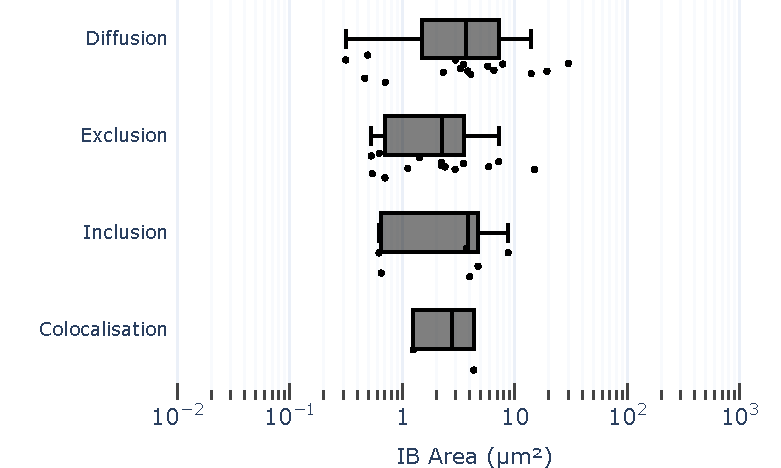
\includegraphics[width=1\linewidth]{09. Chapter 4/Figs/01. pIB/04. IFIT3/02. box_i3_vero.pdf}
    \end{subfigure}
    \caption[Interaction Phenotypes of Monkey IFIT3 with Human pIBs in the Vero Cell Line.]{\textbf{Interaction Phenotypes of Monkey IFIT3 with Human pIBs in the Vero Cell Line.} Vero cells were transfected with hRSV N and P containing plasmids using TransIT-X2 and were fixed after 24 hours. Cells were labeled with anti-RSV N and anti-IFIT3 antibodies and imaged on confocal microscope. Panel (a) shows percentual proportions of observed phenotypes between hRSV pseudo inclusion bodies and monkey IFIT3 (39 observations), with the red dotted line denoting the 5\% threshold, marking phenotypes considered relevant above this limit. Panel (b) shows the IB area in \(\mu \mbox{m}^2\) per observed relevant phenotype.}
    \label{fig:Interaction Phenotypes of Monkey IFIT3 with Human pIBs in the VERO Cell Line}
\end{figure}

\begin{figure}
    \centering
    \includegraphics[width=1\linewidth]{09. Chapter 4/Figs/01. pIB/04. IFIT3/03. i3-vero-hnhp.pdf}
    \caption[Representative Images of Interaction Phenotypes of Monkey IFIT3 with Human pIBs in the Vero Cell Line.]{\textbf{Representative Images of Interaction Phenotypes of Monkey IFIT3 with Human pIBs in the Vero Cell Line.} Vero cells were transfected with hRSV N and P containing plasmids using TransIT-X2 and were fixed after 24 hours. Cellular nuclei were stained with DAPI (yellow), and cells were double-labeled with anti-RSV N (cyan) and anti-IFIT3 (magenta) antibodies. This figure showcases representative examples of relevant phenotypes in the interaction between monkey IFIT3 and hRSV pseudo inclusion bodies. These phenotypes are presented in descending order based on their percentage proportions. The scale bar indicates 2 \(\mu \mbox{m}\).}
    \label{fig:Representative Images of Interaction Phenotypes of Monkey IFIT3 with Human pIBs in the VERO Cell Line}
\end{figure}

Next we investigated IFIT3 interaction with RSV pseudo incluson bodies. As mentioned above we failed to generate samples concisting either of HEK293T cells transfected with hRSV N and P, or Vero cells transfected with bRSV N and P, which would be also stained for IFIT3. Hence we only present the monkey IFIT3 interaction analysis with hRSV pIBs. The frequencies of observed phenotypes within the 39 observations along with the measured pIB sizes per phenotype which occur with more than 5\% frequency are shown in Figure \ref{fig:Interaction Phenotypes of Monkey IFIT3 with Human pIBs in the VERO Cell Line}. The representative images of phenotypes which occur with at  least 5\% frequency are shown in Figure \ref{fig:Representative Images of Interaction Phenotypes of Monkey IFIT3 with Human pIBs in the VERO Cell Line}. The most prevalent phenotype is diffusn throught the pIB structure, which occured at 41\% of observation. This was closely followed by an exclusion phenotype, which occured at 36\% of observations. We have observed monkey IFIT3 to be forming intra pIB inclusion in 15\% of the cxases. Laslty, 5\% of observations showed colocalisation phenotype, while 3\% of all observations shopwed colocalisation associated with exclusion. With regards of the size profile of the IBs associated with the different phenotyeps which displayed at least 5\% frequency, their median values seem to be quite similar, however they encompass a progressivelymore narrow range of values as the occurance frequency decreases. In more detail the diffusion phenotype median pIB size was 4 \(\mu \mbox{m}^2\) and it encompasses values from 0.3 \(\mu \mbox{m}^2\) to 30 \(\mu \mbox{m}^2\). The exclusion phenotype-associated median area value was 2 \(\mu \mbox{m}^2\), while the range of sizes of the detected pIBs encompassed sub 0.6 \(\mu \mbox{m}^2\) to supra 10 \(\mu \mbox{m}^2\). The size values of inclusion-associated pIBs clustered at around 3 \(\mu \mbox{m}^2\) and ranged from two observations at 6 \(\mu \mbox{m}^2\) to one observation at 9 \(\mu \mbox{m}^2\). Lastly, the pIBs associated with the colocalisation phenotype were of 1.3 \(\mu \mbox{m}^2\) and 4.3 \(\mu \mbox{m}^2\). It seems like predominantly in most cases monkey IFIT3 is not directly seen interacting with the hRSV pIB structures, however in a quater of the cases it seems to be either forming inclusions or being associated with the edge of the pIB strucutre. This data seems to confirm our earlier investigation where IFIT3 exhibited predominantly exclusion and diffusion phenotypes during RSV infection.

\begin{figure}
    \begin{subfigure}{0.495\textwidth}
        \caption{}
        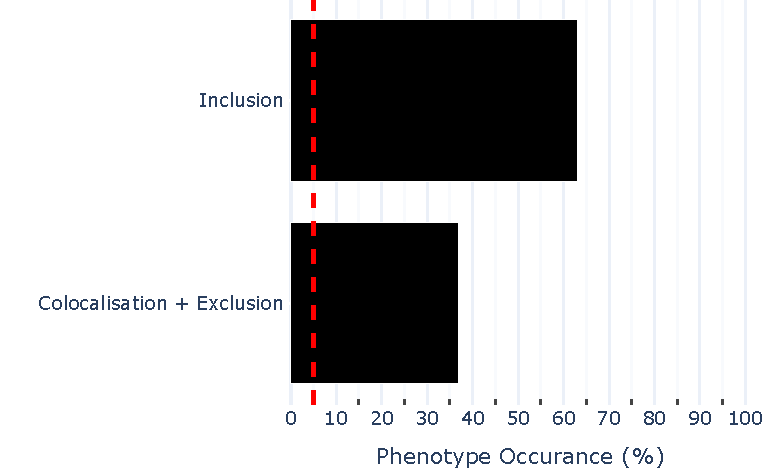
\includegraphics[width=1\linewidth]{09. Chapter 4/Figs/01. pIB/05. IFIT5/01. bar_i5_vero.pdf} 
    \end{subfigure}
    \begin{subfigure}{0.495\textwidth}
        \caption{}
        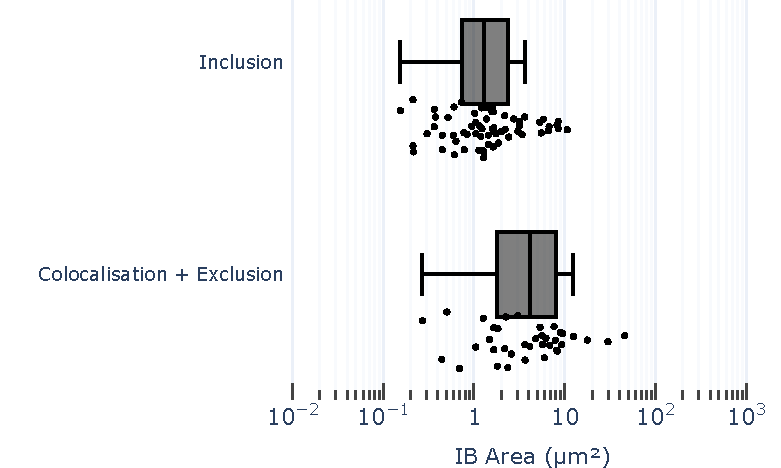
\includegraphics[width=1\linewidth]{09. Chapter 4/Figs/01. pIB/05. IFIT5/02. box_i5_vero.pdf}
    \end{subfigure}
    \caption[Interaction Phenotypes of Monkey IFIT5 with Human pIBs in the Vero Cell Line.]{\textbf{Interaction Phenotypes of Monkey IFIT5 with Human pIBs in the Vero Cell Line.} Vero cells were transfected with hRSV N and P containing plasmids using TransIT-X2 and were fixed after 24 hours. Cells were labeled with anti-RSV N and anti-IFIT5 antibodies and imaged on confocal microscope. Panel (a) shows percentual proportions of observed phenotypes between hRSV pseudo inclusion bodies and monkey IFIT5 (100 observations), with the red dotted line denoting the 5\% threshold, marking phenotypes considered relevant above this limit. Panel (b) shows the IB area in \(\mu \mbox{m}^2\) per observed relevant phenotype.}
    \label{fig:Interaction Phenotypes of Monkey IFIT5 with Human pIBs in the VERO Cell Line}
\end{figure}

\begin{figure}
    \centering
    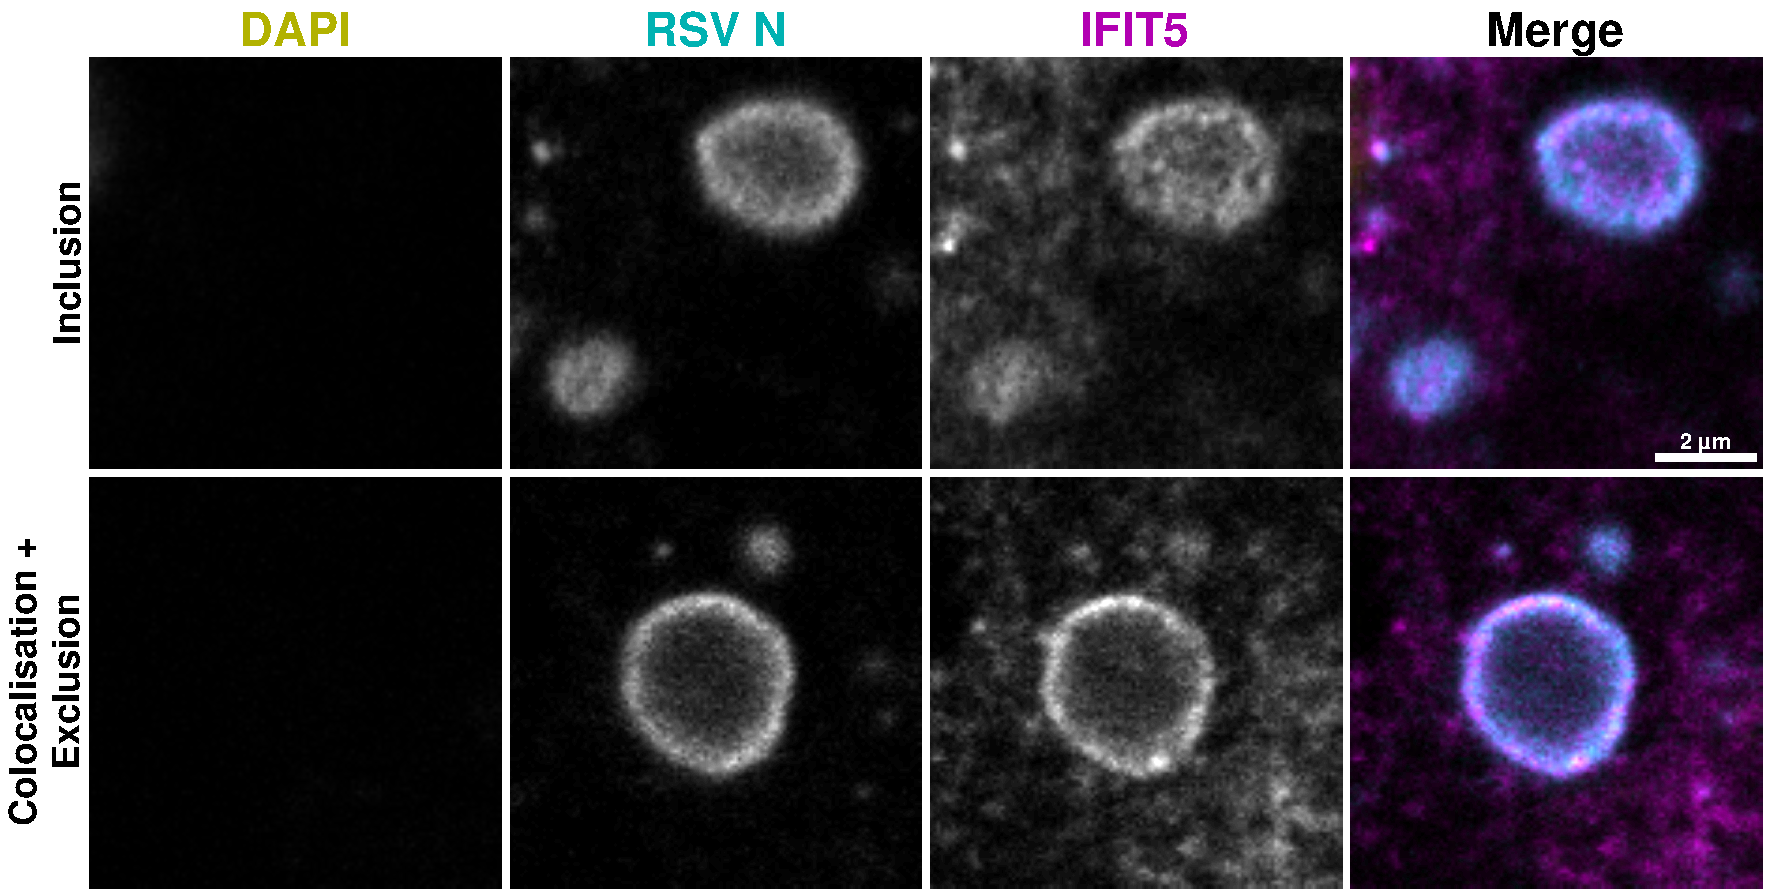
\includegraphics[width=1\linewidth]{09. Chapter 4/Figs/01. pIB/05. IFIT5/03. i5-vero-hnhp.pdf}
    \caption[Representative Images of Interaction Phenotypes of Monkey IFIT5 with Human pIBs in the Vero Cell Line.]{\textbf{Representative Images of Interaction Phenotypes of Monkey IFIT5 with Human pIBs in the Vero Cell Line.} Vero cells were transfected with hRSV N and P containing plasmids using TransIT-X2 and were fixed after 24 hours. Cellular nuclei were stained with DAPI (yellow), and cells were double-labeled with anti-RSV N (cyan) and anti-IFIT5 (magenta) antibodies. This figure showcases representative examples of relevant phenotypes in the interaction between monkey IFIT5 and hRSV pseudo inclusion bodies. These phenotypes are presented in descending order based on their percentage proportions. The scale bar indicates 2 \(\mu \mbox{m}\).}
    \label{fig:Representative Images of Interaction Phenotypes of Monkey IFIT5 with Human pIBs in the VERO Cell Line}
\end{figure}

Lastly we have investigated the IFIT5 interactions with the simplified system of RSV pseudo inclusion bodies. As mentioned previously we only managed to obtain data from Vero cell line transfected with hRSV N and P containing plasmids and thus we can only investigate the monkey IFIT5 interaction with the human pIBs. Figure \ref{fig:Interaction Phenotypes of Monkey IFIT5 with Human pIBs in the VERO Cell Line} shows the frequencies of occurances of the observed phenotypes alongside the measured pIB areas per observed phenotype from the 100 observations that were recorded. Figure \ref{fig:Representative Images of Interaction Phenotypes of Monkey IFIT5 with Human pIBs in the VERO Cell Line} shows the representative images of these pehnotypes. We have observed monkey IFIT5 to exert two hRSV pIB interaction phenotypes i.e. to be forming intra-pIB inclusion or to colocalise with the pIB boundry while being excluded from the pIB structure. The former occured in 62\% of observations, while the latter occured in 38\% of observations. The size of inclusion-associated hRSV pIBs ranged from 0.13 \(\mu \mbox{m}^2\) to 10 \(\mu \mbox{m}^2\), with atypiocal value of 1.2 \(\mu \mbox{m}^2\). On the other hand the size profile of pIBs associated with colocalisation acompalied by exclusion phenotype ranged from 0.23 \(\mu \mbox{m}^2\) to supra 40 with the median value of 4 \(\mu \mbox{m}^2\). There seams to be a differentiation of these pIBs based on size although there is a marked overlap of sizes where both phenotypes occur (between 0.23 and 10 \(\mu \mbox{m}^2\)). Interestingly, previously we have observed both human and bovine IFIT5 to be minimaly interacting with the RSV IBs, with the most prevalent observed phenotype being exclusion (Chapter \ref{ch:Subcellular Localisation of Endogenous IFIT Proteins in the Context of RSV Inclusion Bodies}). We have observed the inclusion phenotype only in 10\% of observations in MDBK cell line and the colocalisation associated with exclusioin phenotype in 5\% of observations in A549 cell line. This suggest that IFIT5 has a propensity to interact with the pseudo inclusion bodies but some factors that are present in RSV IBs during infection are preventing IFIT5 from accessing these structures.

Overall the investigaton of IFIT1, IFIT3, and IFIT5 localisation with regards to the simplified model of RSV inclusion bodies using ectopically expressed pseudo-inclusion bodies yielded somewhat interesting results, which can lead us to uncover the nature of thier interactions and the potential factors that are impeeding these intreactions during RSV infection. With regards to endogenous IFIT1, we have observed minimal interaction in human cells (HEK293T) with hRSV pIBs, although this could have been as a result of size bias of the observed pIBs. We base this assumption based on the observed monkey IFIT1 interactions with human RSV pIBs, where the strong interaction phenotypes (inclusion and colocalisation) correlated with increased pIB size, and especially based on the results from monkey IFIT1 interaction with bovine RSV pIBs where we solely observed phenotypes implying interaction. The monkey IFIT1 data supports the observations from Section \ref{subsec:Endogenous IFIT Interaction with RSV Inclusion Bodies}, where we have observed both human and bovine IFIT1 show strong interaction phenotypes (incluson or colocalisation) with RSV IBs during infection. However this was not the domiminant phenotype observed, which was exclusion. Clearly IFIT1 has a propensity to directly associate with the pIB, a process which seems to be disrupted during infection. Monkey IFIT3 displayed data consistent to what was observed in RSV infection data i.e. majority of the cases being either indirectly associated with pIBs (diffusion), or being excluded from the structures, while directly associating with these strucutres with small but considerable frequency. This suggest that the IFIT3-IB intreraction is directied via biophysical interactions with the pIB and IB structures. Lastly, monkey IFIT5 showed only strong interaction phenotypes with human pIBs. This is unexpected as during infection neither human nor bovine IFIT5 exhibited minimal direct or indirect interaction phenotypes, with the dominant observed phenotype being exclusion. This discrepancy could be due to the diffrential propensity of monkey IFIT5 for interaction with (p)IBs compared to human and bovine IFIT5, or it could mean that viral  or cellular factors associated with and influencing the RSV IBs during infection prevent IFIT5 from interaction with these structures. Overall while these experiments provided us with valuable data that confirmed ourprevious observations (as is the case for IFIT3, or IFIT1 interacting with human pIBs), it has also yielded data which is inconbsistent with previous observations. The other issue is that majority of the gathered data is based on monkey IFITs which are not relevant for human and bovine RSV infection \textit{in vivo}. Thus it is esential that these data is further validated and investrigated using human and bovine IFITs. To do this we aimed to analyse the interaction profiles of exogenbously expressed human and bovine IFITs in the context of human and bovine RSV infection.

\subsection{Overexpressed IFIT1, IFIT3, and IFIT5 During RSV Infection} \label{subsec:Overexpressed IFIT1, IFIT3, and IFIT5 During RSV Infection}
In order to validate the interaction results of monkey IFIT1, IFIT3, and IFIT5 with pseudo IBs and to investigate the maximal potential for intereactions between human and bovine IFIT1, IFIT3, and IFIT5 with human and bovine IBs in the context of infection, we further aimed to conduct IFIT overexpression expreiments coupled with RSV infection. We wanted to decrease the likelihood of nonspecific antibody staining by overexpressing FLAG-tagged IFIT proteins, which would be visualised using monoclonal anti-FLAG antibody. The usage of FLAG tag would allow for higher specificity and increased access for IB detection inside of the phase separated structures \cite{Munro1984Use70.}. To do this we needed a library of FLAG-tagged human and bovine IFIT proteins, cloned in plasmids which allow for effcient translation in transfected cells. We were kindly provided with human IFIT1, IFIT2, IFIT3, and IFIT5 ORF-containng plasmids, each tagged with FLAG in the C terminus by the Viral Gene Expressioin group from the Pirbright Institute. This group also provided a control GFP-FLAG pcDNA3.1 plasmid, which was used as a control for transfection efficiency and persistance. These were already present in a  pcDNA3.1 backbone, whcih was directly suitable for our downstream analyses. We were also kindly provided by bovine IFIT-containing plasmids by CVR Glasgow as a part of their bovine ISG plasmid library. There plasmids were consisting of SCRPSY backbone, which is optimasied for creating lentiviral praticles, and untagged bovine IFIT ORFs. Due to this reason we needed to clone these ORF into pcDNA3.1 plasmid backbone, while cocurently adding a C-terminal FLAG tag.

The schematics and decriptions of the pcDNA3.1 and SCRPSY plasmids are depicted in Section \ref{subsec:DNA Plasmids}, while the detailed description of cloning and subcling methodologies are shown in Section \ref{subsec:PCR for Cloning into pcDNA3.1} and Section \ref{subsec:Common Subcloning Methodologies} respectively. Briefly, we have designed forwards and reverse primers, specific for each bovine \textit{IFITs}, consisting of, among other elements, section of the ORF, FLAG tag, start or stop sequence, and the recognition sites of Acc65I and NotI restriction enzymes respectively. These were specificaly selected as their restrictioni sites are not preset within either of the bovine \textit{IFIT} sequence. These primers were used to PCR amplify and isolate the bovine \textit{IFIT} ORFs from the SCRPSY plasmids. These linear ORFs were subsequently subcloned into the pcDNA3.1 plasmid backbones.

To assay the subcellular localisation of exogenously expressed human and bovine IFIT proteins with regards to human and bovine RSV inclusion bodies, we have transfected the cells with 1 \(\mu\)g per well of a 24 well plate using TransIT-X2, as decribed in Section \ref{subsec:Transfecting Cells}, and infected the cells with MOI 1 RSV based on the standard methodology (described in Section \ref{subsec:Viral Infections, UV-Inactivation and Ruxolitinib Treatment}). There is an inherent difficulty in establishing cocurrent infection and transfection in the same cells, as doing one treatment usually puts the cell in a antiviral state, that prevents further treatment (infection or transfection). Due to this, we have to tried several methodologies to cause cocurrent infection and transfection. To obtain data that would be comparable with the data previously gathered from infectiion experiments (Chapter \ref{ch:Subcellular Localisation of Endogenous IFIT Proteins in the Context of RSV Inclusion Bodies}) i.e. RSV infection that is terminated 24 HPI, we have initialy tried cell transfection, that was follwed by RSV infection 24 hours post transfection. We used the GFP-FLAG control plasmid to easily assess transfection efficiency and persistance, while we have examined the cells for RSV cytophatic effect (e.g. syncytia formation) to confirm sucessful infection. While we were able to detect sucesful transfection 24 hours post transfection, after 24 hours of subvsequent infection none GFP-expression was detected. Next, we have tried simultanoues infection and transfection. This was done by initial inoculatyion of the cells with a virus preparation and incubation with this innoculum for an hour. Afterwards the inoculum was removed, the cells washed with PBS, after which the trabsfection mixture was added in the cell culture media. This however also resulted in minimal GFP expression. In both of these methodologies we have observed robust infection. Lastly we have emplyed initial RSV infection, followed by transfection 24 HPI. The cells were fixed 24 hours post transfection i.e. 48 hours post infection. This methogology yielded the best co-transfection/infection out of all methodologies tried. Saying this, it was still sub optimal as for some IFIT/RSV conbinations we have only detected 10-15 co-transfection/infection cells, although sufficient for confocal microscopy analysis.

This is to be expected as we know that overexpressed hIFIT1, hIFIT2, and hIFIT3 are antiviral against RSV and thus cells that would present ectopicaly expressded IFITs would therefore create an enviroment that would be unbsuitable for RSV life cycle. Along to this and as mantioned above, infected cells activate their innate antiviral pahtwasys and thus prevent another infection or transfection. This creates inherent bias whereby the cells which have the propensity to be coccurently infected and transfected are not representative of the general cellular population. With regards to the lenght of the infection, after 48 HPI we can expect the size of the IBs to be substantialy larger to what we observed at 24 HPI previously. It is reported in the literature that the mean 2D area of bRSV incusion bodies increased from 8.99 \(\mu \mbox{m}^2\) to 22.18 \(\mu \mbox{m}^2\) between 24 HPI and 48 HPI \cite{Jobe2021BovineResponses}. This would thus make it difficult to compare the co-infection/transfection data to the infection data from Chapter \ref{ch:Subcellular Localisation of Endogenous IFIT Proteins in the Context of RSV Inclusion Bodies}. We could however use the present data to investigate the potential influence of ectopicaly expressed IFIT proteins on the 2D IB area, which could be used to gauge the potential anti-RSV mechanism of these proteins. We experienced difficulties in obtaining co-transfection/infection data with several plasmids. These include bovine IFIT1, human IFIT3, and bovine IFIT5. These were possibly die to a variety of reasons e.g. decreased teransfection efficiency due to contaminats present in the plasmid preparation or the tranfection complexex failing to form properly. All of the data presented below is supported by z-stack measurements.

\begin{figure}
    \begin{subfigure}{0.495\textwidth}
        \caption{}
        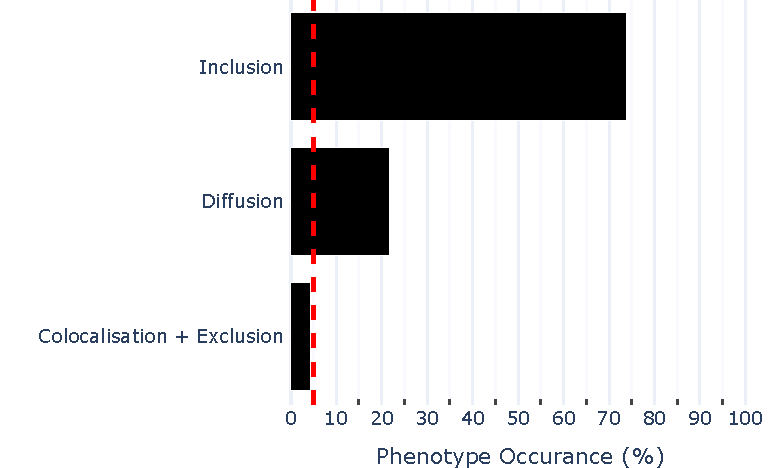
\includegraphics[width=1\linewidth]{09. Chapter 4/Figs/02. Overexpression/01. IFIT1/01. bar_i1_hrsv.pdf} 
    \end{subfigure}
    \begin{subfigure}{0.495\textwidth}
        \caption{}
        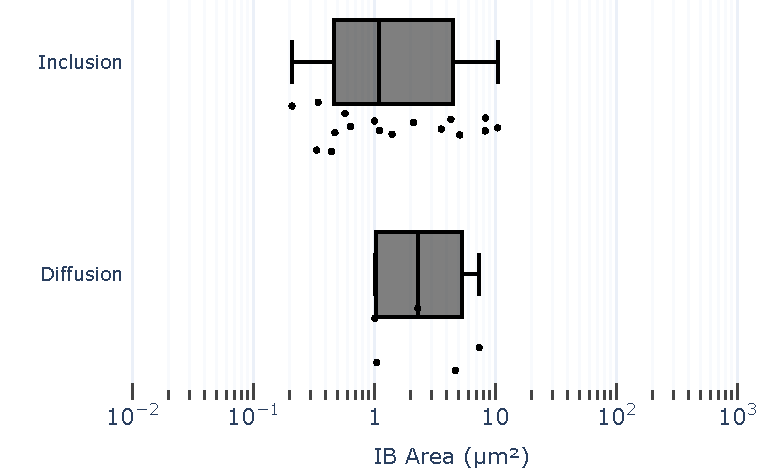
\includegraphics[width=1\linewidth]{09. Chapter 4/Figs/02. Overexpression/01. IFIT1/02. box_i1_hrsv.pdf}
    \end{subfigure}
    \caption[Observed Phenotypes of Exogenous hIFIT1 in the Context of hRSV Inclusion Bodies in Vero Cell Line.]{\textbf{Observed Phenotypes of Exogenous hIFIT1 in the Context of hRSV Inclusion Bodies in Vero Cell Line.} Vero cells were infected with human RSV at MOI 1. 24 HPI, the cells were transfected with hIFIT1-FLAG containing plasmids using TransIT-X2 and were fixed after a further 24 hours. Cells were labelled with anti-RSV N and anti-FLAG antibodies and imaged on a confocal microscope. Panel (a) shows the percentual proportions of observed phenotypes between hRSV inclusion bodies and exogenous hIFIT1 (23 observations), with the red dotted line denoting the 5\% threshold, marking phenotypes considered relevant above this limit. Panel (b) shows the IB area in \(\mu \mbox{m}^2\) per observed relevant phenotype.}
    \label{fig:Observed Phenotypes of Exogenous hIFIT1 in the Context of hRSV Inclusion Bodies in VERO Cell Line}
\end{figure}

\begin{figure}
    \centering
    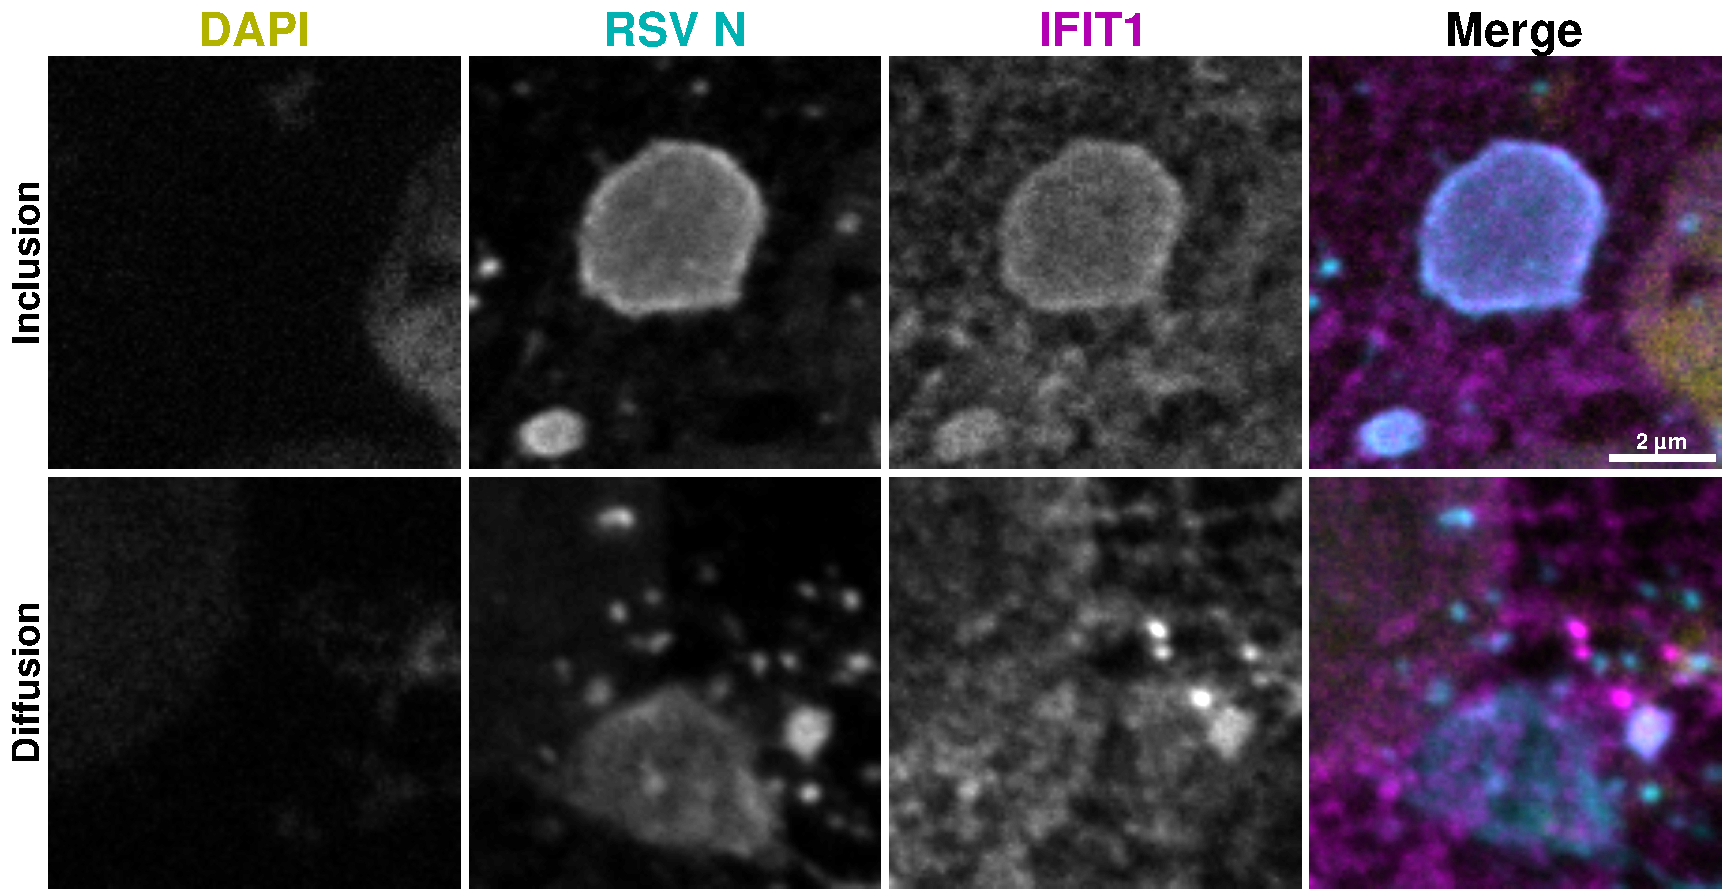
\includegraphics[width=1\linewidth]{09. Chapter 4/Figs/02. Overexpression/01. IFIT1/03. i1-hrsv.pdf}
    \caption[Representative Images of Observed Phenotypes of Exogenous hIFIT1 in the Context of hRSV Inclusion Bodies in Vero Cell Line.]{\textbf{Representative Images of Observed Phenotypes of Exogenous hIFIT1 in the Context of hRSV Inclusion Bodies in Vero Cell Line.} Vero cells were infected with human RSV at MOI 1. 24 HPI, the cells were transfected with hIFIT1-FLAG containing plasmids using TransIT-X2 and were fixed after a further 24 hours. Cellular nuclei were stained with DAPI (yellow), and cells were double-labelled with anti-RSV N (cyan) and anti-FLAG (magenta) antibodies. This figure showcases representative examples of relevant phenotypes in the interaction between exogenous hIFIT1 and hRSV inclusion bodies. These phenotypes are presented in descending order based on their percentage proportions. The scale bar indicates 2 \(\mu \mbox{m}\).}
    \label{fig:Representative Images of Observed Phenotypes of Exogenous hIFIT1 in the Context of hRSV Inclusion Bodies in VERO Cell Line}
\end{figure}

We have observed 23 instances of human IFIT1 being expressed in hRSV infected cells. The frequencies of occurances of observed phenotypes along to the measured IB sizes of phenotypes occuring with >5\% fruequency are shown in Figure \ref{fig:Observed Phenotypes of Exogenous hIFIT1 in the Context of hRSV Inclusion Bodies in VERO Cell Line}. The representative images of the latter are shown in Figure \ref{fig:Representative Images of Observed Phenotypes of Exogenous hIFIT1 in the Context of hRSV Inclusion Bodies in VERO Cell Line}. 

74 22

1.1 2.2

incl 0.2 1.1 10
diff 1 2.2 7

no ibs above 10 detected (weird)

\begin{figure}
    \begin{subfigure}{0.495\textwidth}
        \caption{}
        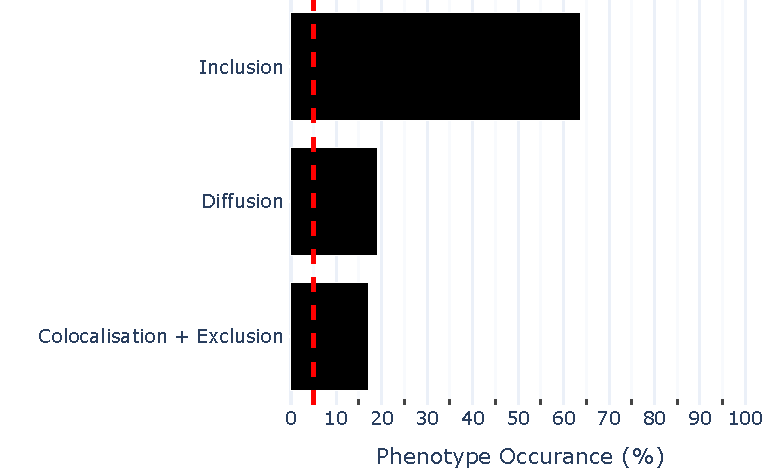
\includegraphics[width=1\linewidth]{09. Chapter 4/Figs/02. Overexpression/01. IFIT1/04. bar_i1_brsv.pdf} 
    \end{subfigure}
    \begin{subfigure}{0.495\textwidth}
        \caption{}
        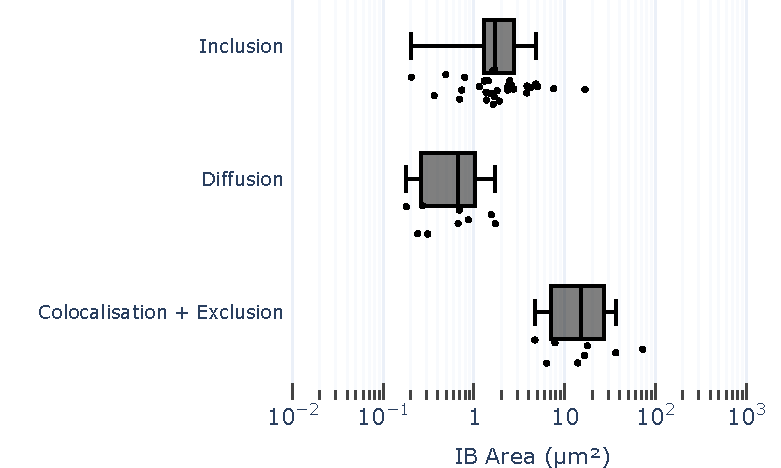
\includegraphics[width=1\linewidth]{09. Chapter 4/Figs/02. Overexpression/01. IFIT1/05. box_i1_brsv.pdf}
    \end{subfigure}
    \caption[Observed Phenotypes of Exogenous hIFIT1 in the Context of bRSV Inclusion Bodies in Vero Cell Line.]{\textbf{Observed Phenotypes of Exogenous hIFIT1 in the Context of bRSV Inclusion Bodies in Vero Cell Line.} Vero cells were infected with bovine RSV at MOI 1. 24 HPI, the cells were transfected with hIFIT1-FLAG containing plasmids using TransIT-X2 and were fixed after further 24 hours. Cells were labeled with anti-RSV N and anti-FLAG antibodies and imaged on confocal microscope. Panel (a) shows percentual proportions of observed phenotypes between bRSV inclusion bodies and exogenous hIFIT1 (47 observations), with the red dotted line denoting the 5\% threshold, marking phenotypes considered relevant above this limit. Panel (b) shows the IB area in \(\mu \mbox{m}^2\) per observed relevant phenotype.}
    \label{fig:Observed Phenotypes of Exogenous hIFIT1 in the Context of bRSV Inclusion Bodies in VERO Cell Line}
\end{figure}

\begin{figure}
    \centering
    \includegraphics[width=1\linewidth]{09. Chapter 4/Figs/02. Overexpression/01. IFIT1/06. i1-brsv.pdf}
    \caption[Representative Images of Observed Phenotypes of Exogenous hIFIT1 in the Context of bRSV Inclusion Bodies in Vero Cell Line.]{\textbf{Representative Images of Observed Phenotypes of Exogenous hIFIT1 in the Context of bRSV Inclusion Bodies in Vero Cell Line.} Vero cells were infected with bovine RSV at MOI 1. 24 HPI, the cells were transfected with hIFIT1-FLAG containing plasmids using TransIT-X2 and were fixed after further 24 hours. Cellular nuclei were stained with DAPI (yellow), and cells were double-labeled with anti-RSV N (cyan) and anti-FLAG (magenta) antibodies. This figure showcases representative examples of relevant phenotypes in the interaction between exogenous hIFIT1 and bRSV inclusion bodies. These phenotypes are presented in descending order based on their percentage proportions. The scale bar indicates 2 \(\mu \mbox{m}\).}
    \label{fig:Representative Images of Observed Phenotypes of Exogenous hIFIT1 in the Context of bRSV Inclusion Bodies in VERO Cell Line}
\end{figure}

64 19 16

1.8, 0.8, 14

0.2 1.8 >10
<0.2 0.8 >1
>5 14 70

% oe bi3
Overexpressed bIFIT3-FLAG was observed to colocalise with hRSV inclusion bodies (top panel; highlighted with arrows), as well as being excluded from the hRSV IBs, without any signs of IFIT3 signal on the periphery of the IB structures (middle and bottom panel). This data is supported by z stack measurements.

\begin{figure}
    \begin{subfigure}{0.495\textwidth}
        \caption{}
        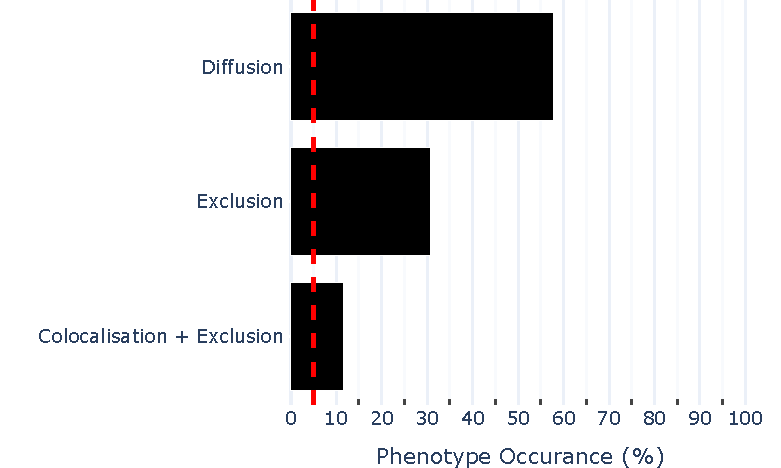
\includegraphics[width=1\linewidth]{09. Chapter 4/Figs/02. Overexpression/03. IFIT3/01. bar_i3_hrsv.pdf} 
    \end{subfigure}
    \begin{subfigure}{0.495\textwidth}
        \caption{}
        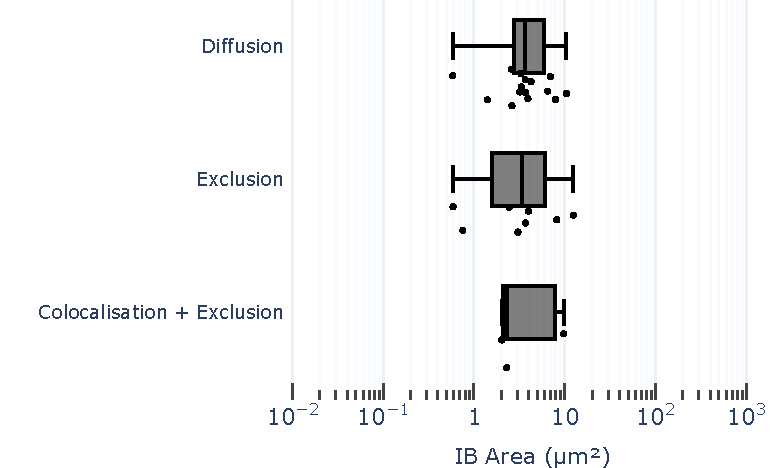
\includegraphics[width=1\linewidth]{09. Chapter 4/Figs/02. Overexpression/03. IFIT3/02. box_i3_hrsv.pdf}
    \end{subfigure}
    \caption[Observed Phenotypes of Exogenous bIFIT3 in the Context of hRSV Inclusion Bodies in Vero Cell Line.]{\textbf{Observed Phenotypes of Exogenous bIFIT3 in the Context of hRSV Inclusion Bodies in Vero Cell Line.} Vero cells were infected with human RSV at MOI 1. 24 HPI, the cells were transfected with bIFIT3-FLAG containing plasmids using TransIT-X2 and were fixed after further 24 hours. Cells were labeled with anti-RSV N and anti-FLAG antibodies and imaged on confocal microscope. Panel (a) shows percentual proportions of observed phenotypes between hRSV inclusion bodies and exogenous bIFIT3 (26 observations), with the red dotted line denoting the 5\% threshold, marking phenotypes considered relevant above this limit. Panel (b) shows the IB area in \(\mu \mbox{m}^2\) per observed relevant phenotype.}
    \label{fig:Observed Phenotypes of Exogenous bIFIT3 in the Context of hRSV Inclusion Bodies in VERO Cell Line}
\end{figure}

\begin{figure}
    \centering
    \includegraphics[width=1\linewidth]{09. Chapter 4/Figs/02. Overexpression/03. IFIT3/03. bi3-hrsv.pdf}
    \caption[Representative Images of Observed Phenotypes of Exogenous bIFIT3 in the Context of hRSV Inclusion Bodies in Vero Cell Line.]{\textbf{Representative Images of Observed Phenotypes of Exogenous bIFIT3 in the Context of hRSV Inclusion Bodies in Vero Cell Line.} Vero cells were infected with human RSV at MOI 1. 24 HPI, the cells were transfected with bIFIT3-FLAG containing plasmids using TransIT-X2 and were fixed after further 24 hours. Cellular nuclei were stained with DAPI (yellow), and cells were double-labeled with anti-RSV N (cyan) and anti-FLAG (magenta) antibodies. This figure showcases representative examples of relevant phenotypes in the interaction between exogenous bIFIT3 and hRSV inclusion bodies. These phenotypes are presented in descending order based on their percentage proportions. The scale bar indicates 2 \(\mu \mbox{m}\).}
    \label{fig:Representative Images of Observed Phenotypes of Exogenous bIFIT3 in the Context of hRSV Inclusion Bodies in VERO Cell Line}
\end{figure}

57 31 12

4, 3.3, 2.1

0.6 4 >10
0.6 3.3 >10
2 2.1 10

Very similar phenotype is observed for overexpressed bIFIT3-FLAG in bRSV infected cells. We see colocalization with IB (top panel) as well as exclusion from the structure without any signs of IFIT3 signal on the periphery of the IB structure (bottom panel). This data is as well supported by z stack measurements.

\begin{figure}
    \begin{subfigure}{0.495\textwidth}
        \caption{}
        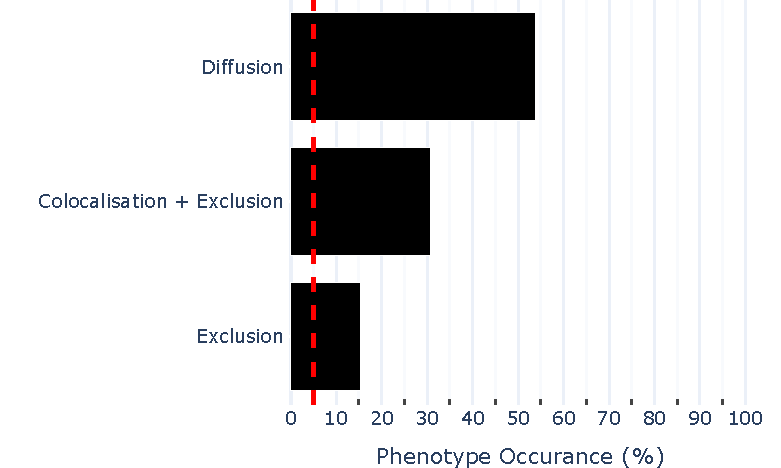
\includegraphics[width=1\linewidth]{09. Chapter 4/Figs/02. Overexpression/03. IFIT3/04. bar_i3_brsv.pdf} 
    \end{subfigure}
    \begin{subfigure}{0.495\textwidth}
        \caption{}
        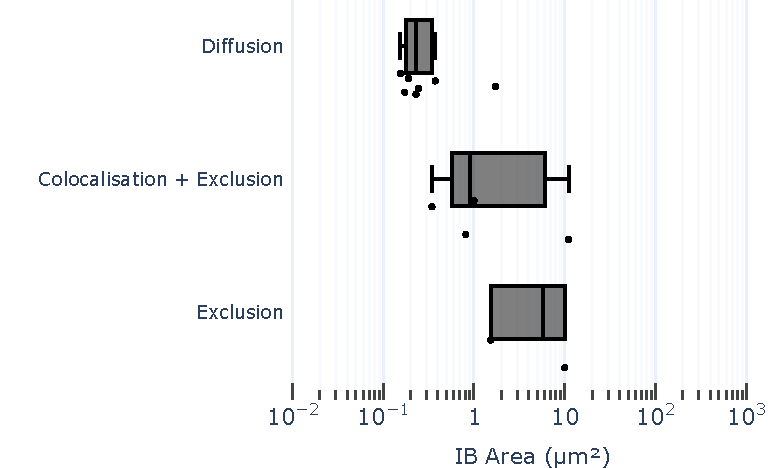
\includegraphics[width=1\linewidth]{09. Chapter 4/Figs/02. Overexpression/03. IFIT3/05. box_i3_brsv.pdf}
    \end{subfigure}
    \caption[Observed Phenotypes of Exogenous bIFIT3 in the Context of bRSV Inclusion Bodies in Vero Cell Line.]{\textbf{Observed Phenotypes of Exogenous bIFIT3 in the Context of bRSV Inclusion Bodies in Vero Cell Line.} Vero cells were infected with bovine RSV at MOI 1. 24 HPI, the cells were transfected with bIFIT3-FLAG containing plasmids using TransIT-X2 and were fixed after further 24 hours. Cells were labeled with anti-RSV N and anti-FLAG antibodies and imaged on confocal microscope. Panel (a) shows percentual proportions of observed phenotypes between bRSV inclusion bodies and exogenous bIFIT3 (13 observations), with the red dotted line denoting the 5\% threshold, marking phenotypes considered relevant above this limit. Panel (b) shows the IB area in \(\mu \mbox{m}^2\) per observed relevant phenotype.}
    \label{fig:Observed Phenotypes of Exogenous bIFIT3 in the Context of bRSV Inclusion Bodies in VERO Cell Line}
\end{figure}

\begin{figure}
    \centering
    \includegraphics[width=1\linewidth]{09. Chapter 4/Figs/02. Overexpression/03. IFIT3/06. bi3-brsv.pdf}
    \caption[Representative Images of Observed Phenotypes of Exogenous bIFIT3 in the Context of bRSV Inclusion Bodies in Vero Cell Line.]{\textbf{Representative Images of Observed Phenotypes of Exogenous bIFIT3 in the Context of bRSV Inclusion Bodies in Vero Cell Line.} Vero cells were infected with bovine RSV at MOI 1. 24 HPI, the cells were transfected with bIFIT3-FLAG containing plasmids using TransIT-X2 and were fixed after further 24 hours. Cellular nuclei were stained with DAPI (yellow), and cells were double-labeled with anti-RSV N (cyan) and anti-FLAG (magenta) antibodies. This figure showcases representative examples of relevant phenotypes in the interaction between exogenous bIFIT3 and bRSV inclusion bodies. These phenotypes are presented in descending order based on their percentage proportions. The scale bar indicates 2 \(\mu \mbox{m}\).}
    \label{fig:Representative Images of Observed Phenotypes of Exogenous bIFIT3 in the Context of bRSV Inclusion Bodies in VERO Cell Line}
\end{figure}

54 31 15

0.22 0.9 6

<0.2 0.22 <2
0.33 0.9 >10
>1 6 10

% oe i5
hIFIT5-FLAG is colocalising with hRSV inclusion bodies (basically resembling the P staining), while in bRSV infected cell there is a hint of IFIT5 signal concentration at the side of bRSV IB.

This data is by single cells per conditions as transfection did not work well. It is however supported by z stack measurements.

\begin{figure}
    \begin{subfigure}{0.495\textwidth}
        \caption{}
        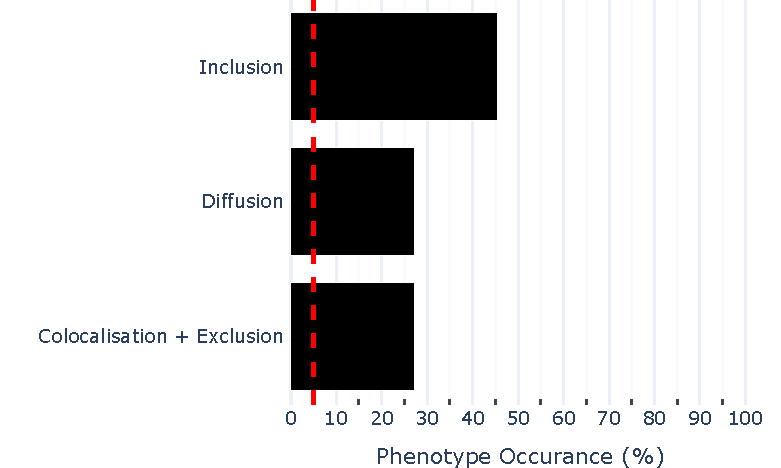
\includegraphics[width=1\linewidth]{09. Chapter 4/Figs/02. Overexpression/04. IFIT5/01. bar_i5_hrsv.pdf} 
    \end{subfigure}
    \begin{subfigure}{0.495\textwidth}
        \caption{}
        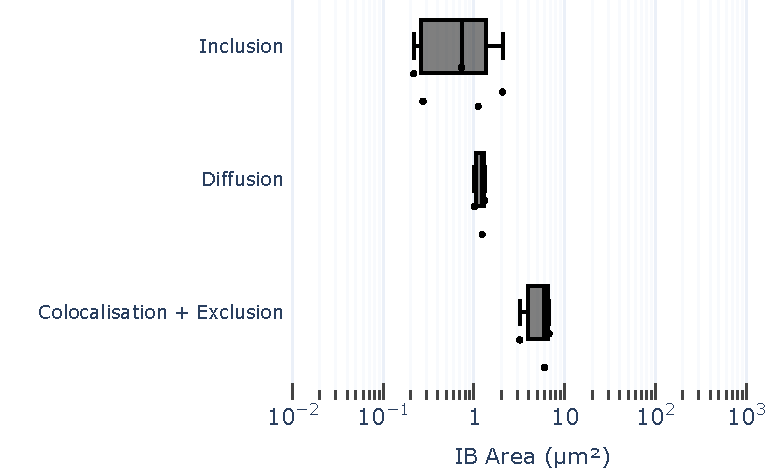
\includegraphics[width=1\linewidth]{09. Chapter 4/Figs/02. Overexpression/04. IFIT5/02. box_i5_hrsv.pdf}
    \end{subfigure}
    \caption[Observed Phenotypes of Exogenous hIFIT5 in the Context of hRSV Inclusion Bodies in Vero Cell Line.]{\textbf{Observed Phenotypes of Exogenous hIFIT5 in the Context of hRSV Inclusion Bodies in Vero Cell Line.} Vero cells were infected with human RSV at MOI 1. 24 HPI, the cells were transfected with hIFIT5-FLAG containing plasmids using TransIT-X2 and were fixed after further 24 hours. Cells were labeled with anti-RSV N and anti-FLAG antibodies and imaged on confocal microscope. Panel (a) shows percentual proportions of observed phenotypes between hRSV inclusion bodies and exogenous hIFIT5 (11 observations), with the red dotted line denoting the 5\% threshold, marking phenotypes considered relevant above this limit. Panel (b) shows the IB area in \(\mu \mbox{m}^2\) per observed relevant phenotype.}
    \label{fig:Observed Phenotypes of Exogenous hIFIT5 in the Context of hRSV Inclusion Bodies in VERO Cell Line}
\end{figure}

\begin{figure}
    \centering
    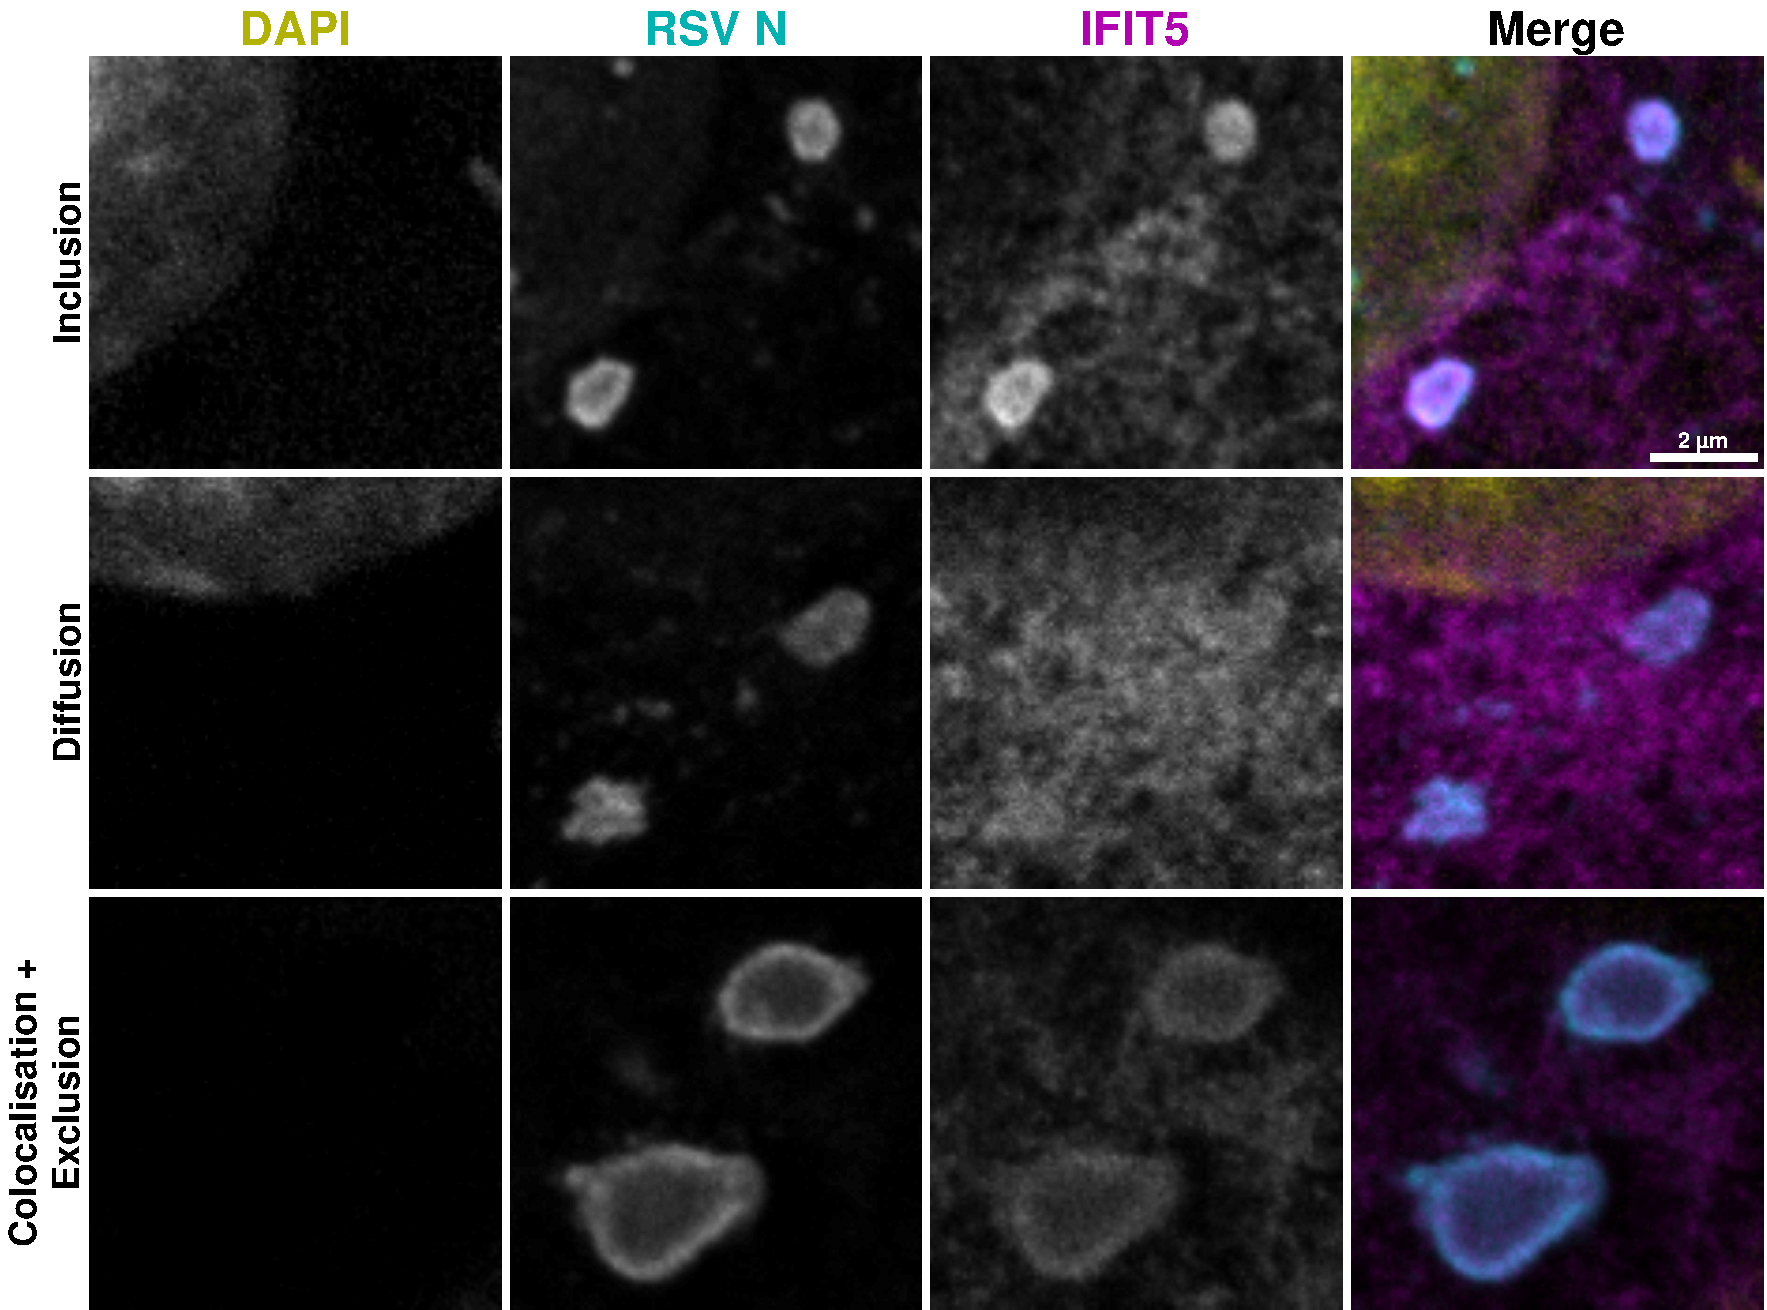
\includegraphics[width=1\linewidth]{09. Chapter 4/Figs/02. Overexpression/04. IFIT5/03. i5-hrsv.pdf}
    \caption[Representative Images of Observed Phenotypes of Exogenous hIFIT5 in the Context of hRSV Inclusion Bodies in Vero Cell Line.]{\textbf{Representative Images of Observed Phenotypes of Exogenous hIFIT5 in the Context of hRSV Inclusion Bodies in Vero Cell Line.} Vero cells were infected with human RSV at MOI 1. 24 HPI, the cells were transfected with hIFIT5-FLAG containing plasmids using TransIT-X2 and were fixed after further 24 hours. Cellular nuclei were stained with DAPI (yellow), and cells were double-labeled with anti-RSV N (cyan) and anti-FLAG (magenta) antibodies. This figure showcases representative examples of relevant phenotypes in the interaction between exogenous hIFIT5 and hRSV inclusion bodies. These phenotypes are presented in descending order based on their percentage proportions. The scale bar indicates 2 \(\mu \mbox{m}\).}
    \label{fig:Representative Images of Observed Phenotypes of Exogenous hIFIT5 in the Context of hRSV Inclusion Bodies in VERO Cell Line}
\end{figure}

45 26 26

0.7 1.2 6

>0.2 0.7 2
1 1.2 1.2
>3 6 7

\begin{figure}
    \begin{subfigure}{0.495\textwidth}
        \caption{}
        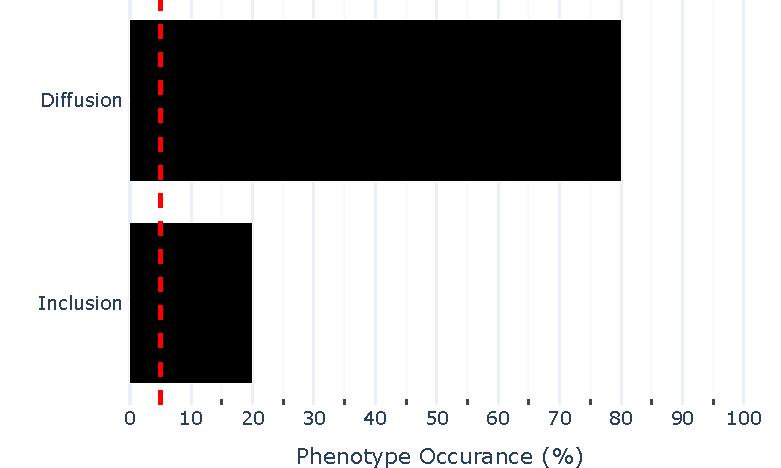
\includegraphics[width=1\linewidth]{09. Chapter 4/Figs/02. Overexpression/04. IFIT5/04. bar_i5_brsv.pdf} 
    \end{subfigure}
    \begin{subfigure}{0.495\textwidth}
        \caption{}
        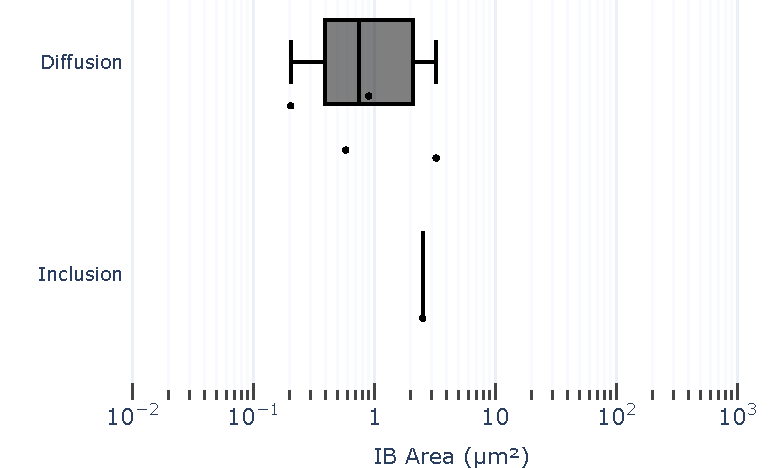
\includegraphics[width=1\linewidth]{09. Chapter 4/Figs/02. Overexpression/04. IFIT5/05. box_i5_brsv.pdf}
    \end{subfigure}
    \caption[Observed Phenotypes of Exogenous hIFIT5 in the Context of bRSV Inclusion Bodies in Vero Cell Line.]{\textbf{Observed Phenotypes of Exogenous hIFIT5 in the Context of bRSV Inclusion Bodies in Vero Cell Line.} Vero cells were infected with bovine RSV at MOI 1. 24 HPI, the cells were transfected with hIFIT5-FLAG containing plasmids using TransIT-X2 and were fixed after further 24 hours. Cells were labeled with anti-RSV N and anti-FLAG antibodies and imaged on confocal microscope. Panel (a) shows percentual proportions of observed phenotypes between bRSV inclusion bodies and exogenous hIFIT5 (5 observations), with the red dotted line denoting the 5\% threshold, marking phenotypes considered relevant above this limit. Panel (b) shows the IB area in \(\mu \mbox{m}^2\) per observed relevant phenotype.}
    \label{fig:Observed Phenotypes of Exogenous hIFIT5 in the Context of bRSV Inclusion Bodies in VERO Cell Line}
\end{figure}

\begin{figure}
    \centering
    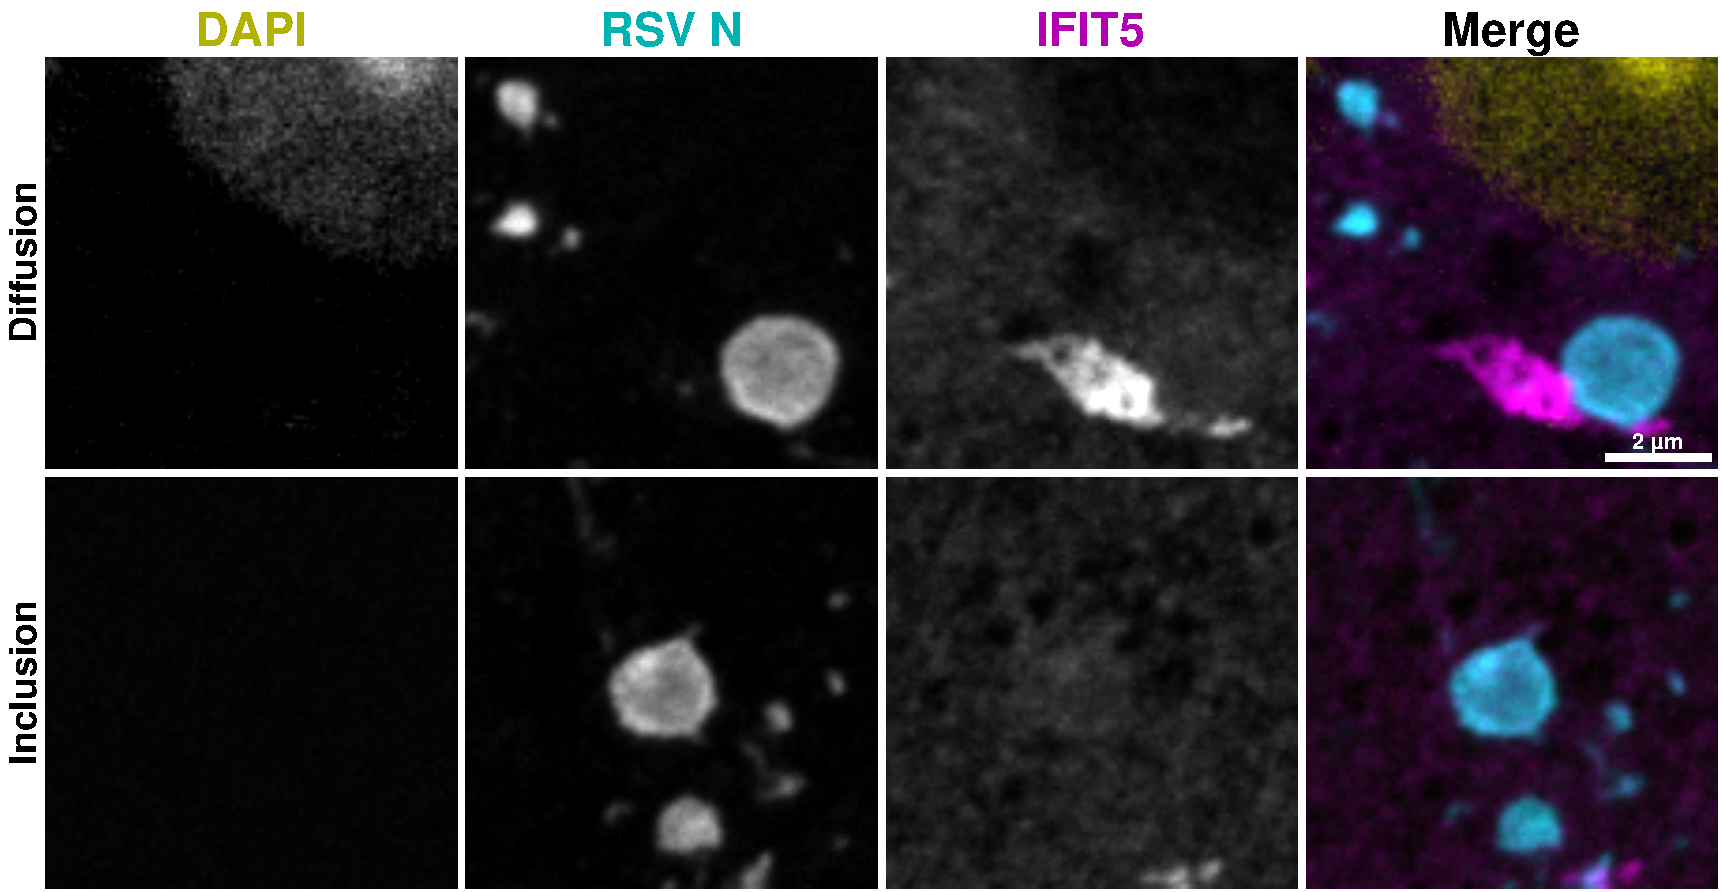
\includegraphics[width=1\linewidth]{09. Chapter 4/Figs/02. Overexpression/04. IFIT5/06. i5-brsv.pdf}
    \caption[Representative Images of Observed Phenotypes of Exogenous hIFIT5 in the Context of bRSV Inclusion Bodies in Vero Cell Line.]{\textbf{Representative Images of Observed Phenotypes of Exogenous hIFIT5 in the Context of bRSV Inclusion Bodies in Vero Cell Line.} Vero cells were infected with bovine RSV at MOI 1. 24 HPI, the cells were transfected with hIFIT5-FLAG containing plasmids using TransIT-X2 and were fixed after further 24 hours. Cellular nuclei were stained with DAPI (yellow), and cells were double-labeled with anti-RSV N (cyan) and anti-FLAG (magenta) antibodies. This figure showcases representative examples of relevant phenotypes in the interaction between exogenous hIFIT5 and bRSV inclusion bodies. These phenotypes are presented in descending order based on their percentage proportions. The scale bar indicates 2 \(\mu \mbox{m}\).}
    \label{fig:Representative Images of Observed Phenotypes of Exogenous hIFIT5 in the Context of bRSV Inclusion Bodies in VERO Cell Line}
\end{figure}

80 20

0.7 2.3

0.2 0.7 >3
2.3

% summary
Overexpressed hIFIT1-FLAG in the context of h/bRSV infection colocalises to both human and bovine IB structures.

Overexpressed bIFIT3 behaves equally between hRSV and bRSV infection, that is it sometimes colocalises with the IB structure and sometimes is completely excluded from the structure.

Overexpressed hIFIT5 in hRSV infected cells colocalises with the IBs.